% !TEX root = ../main.tex
%
\section{Background estimation}

\subsection{Measurement of the QCD OS/SS factor}\label{suppsec:fits}

\subsubsection{\etau{} channel}

\begin{figure}[h!]
    \centering
    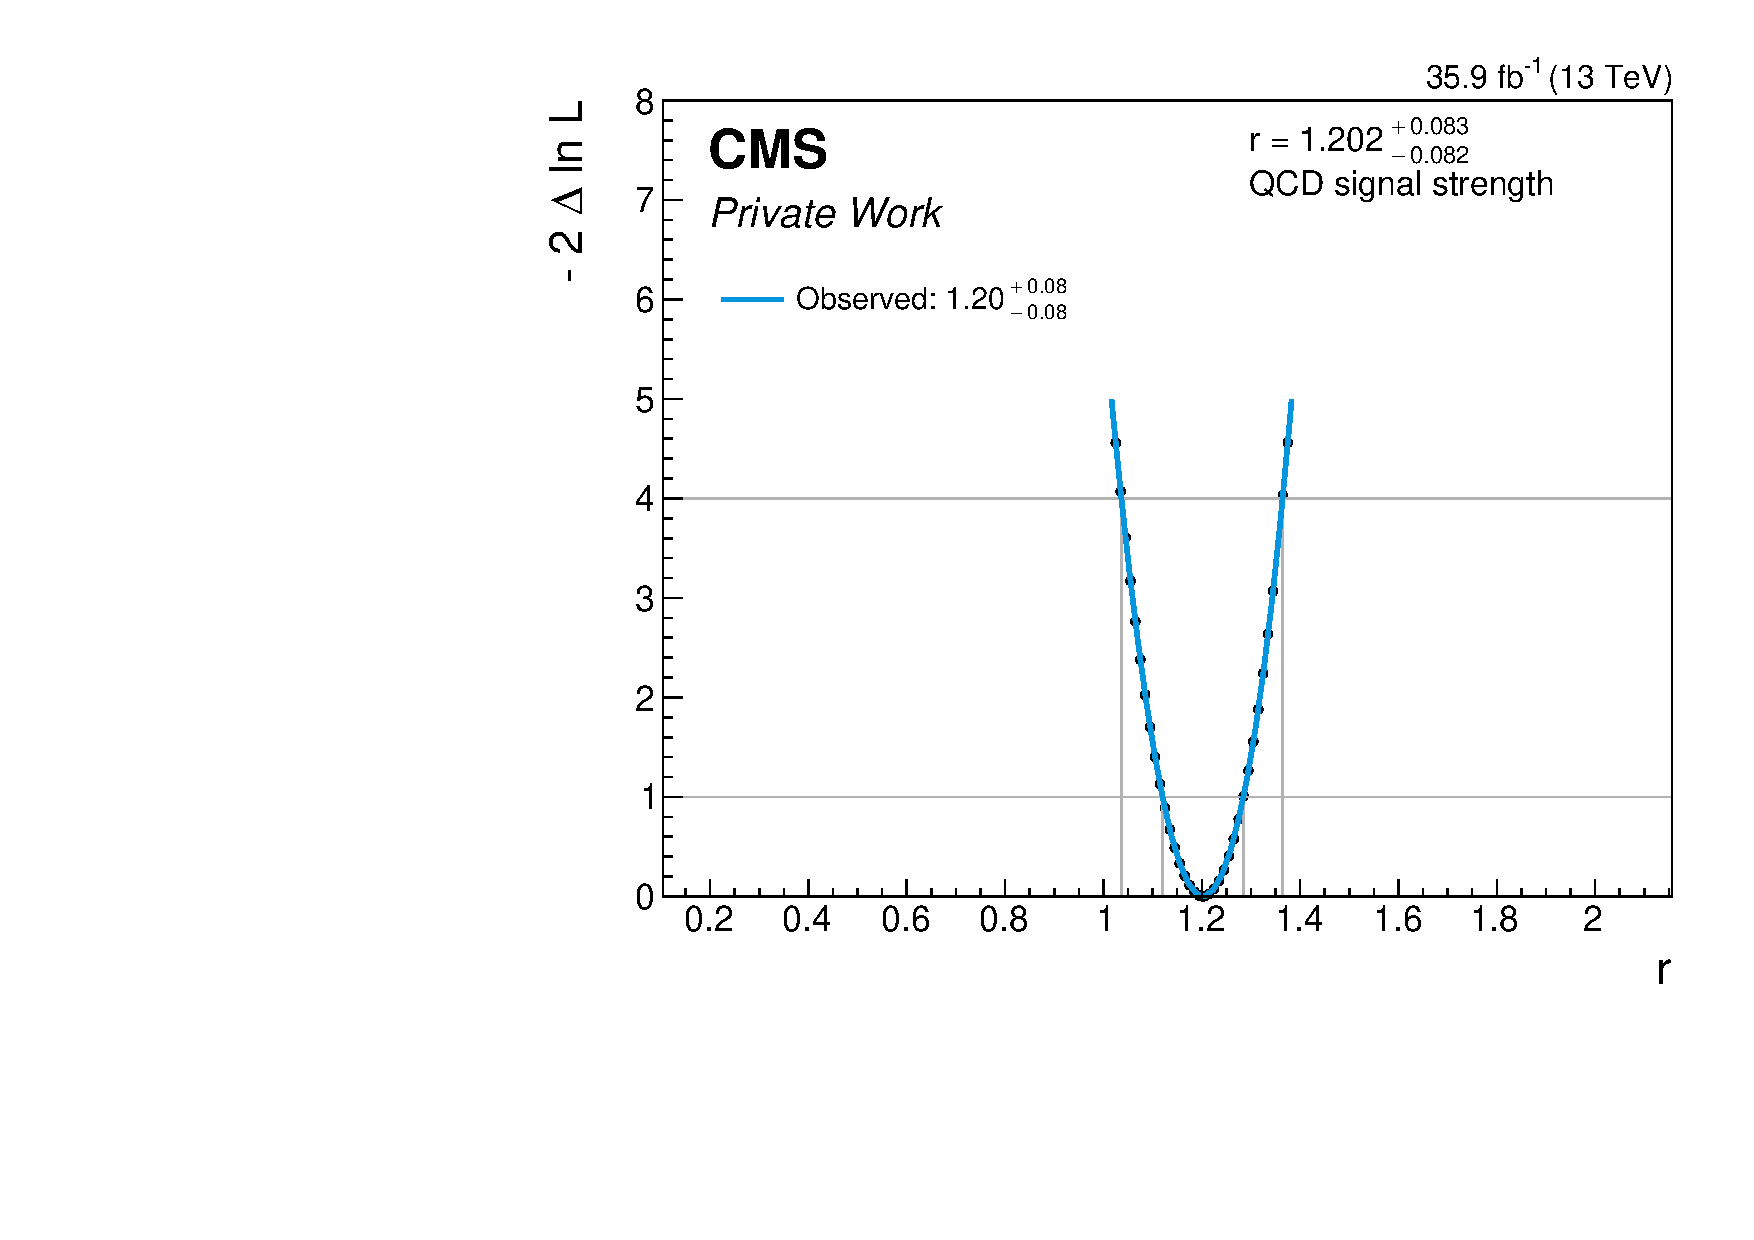
\includegraphics[width=.49\textwidth]{Figures/background_estimation/RQCDOSSS/Scans/et_ZeroJet2D_antiiso_near/plots/nll.pdf}
    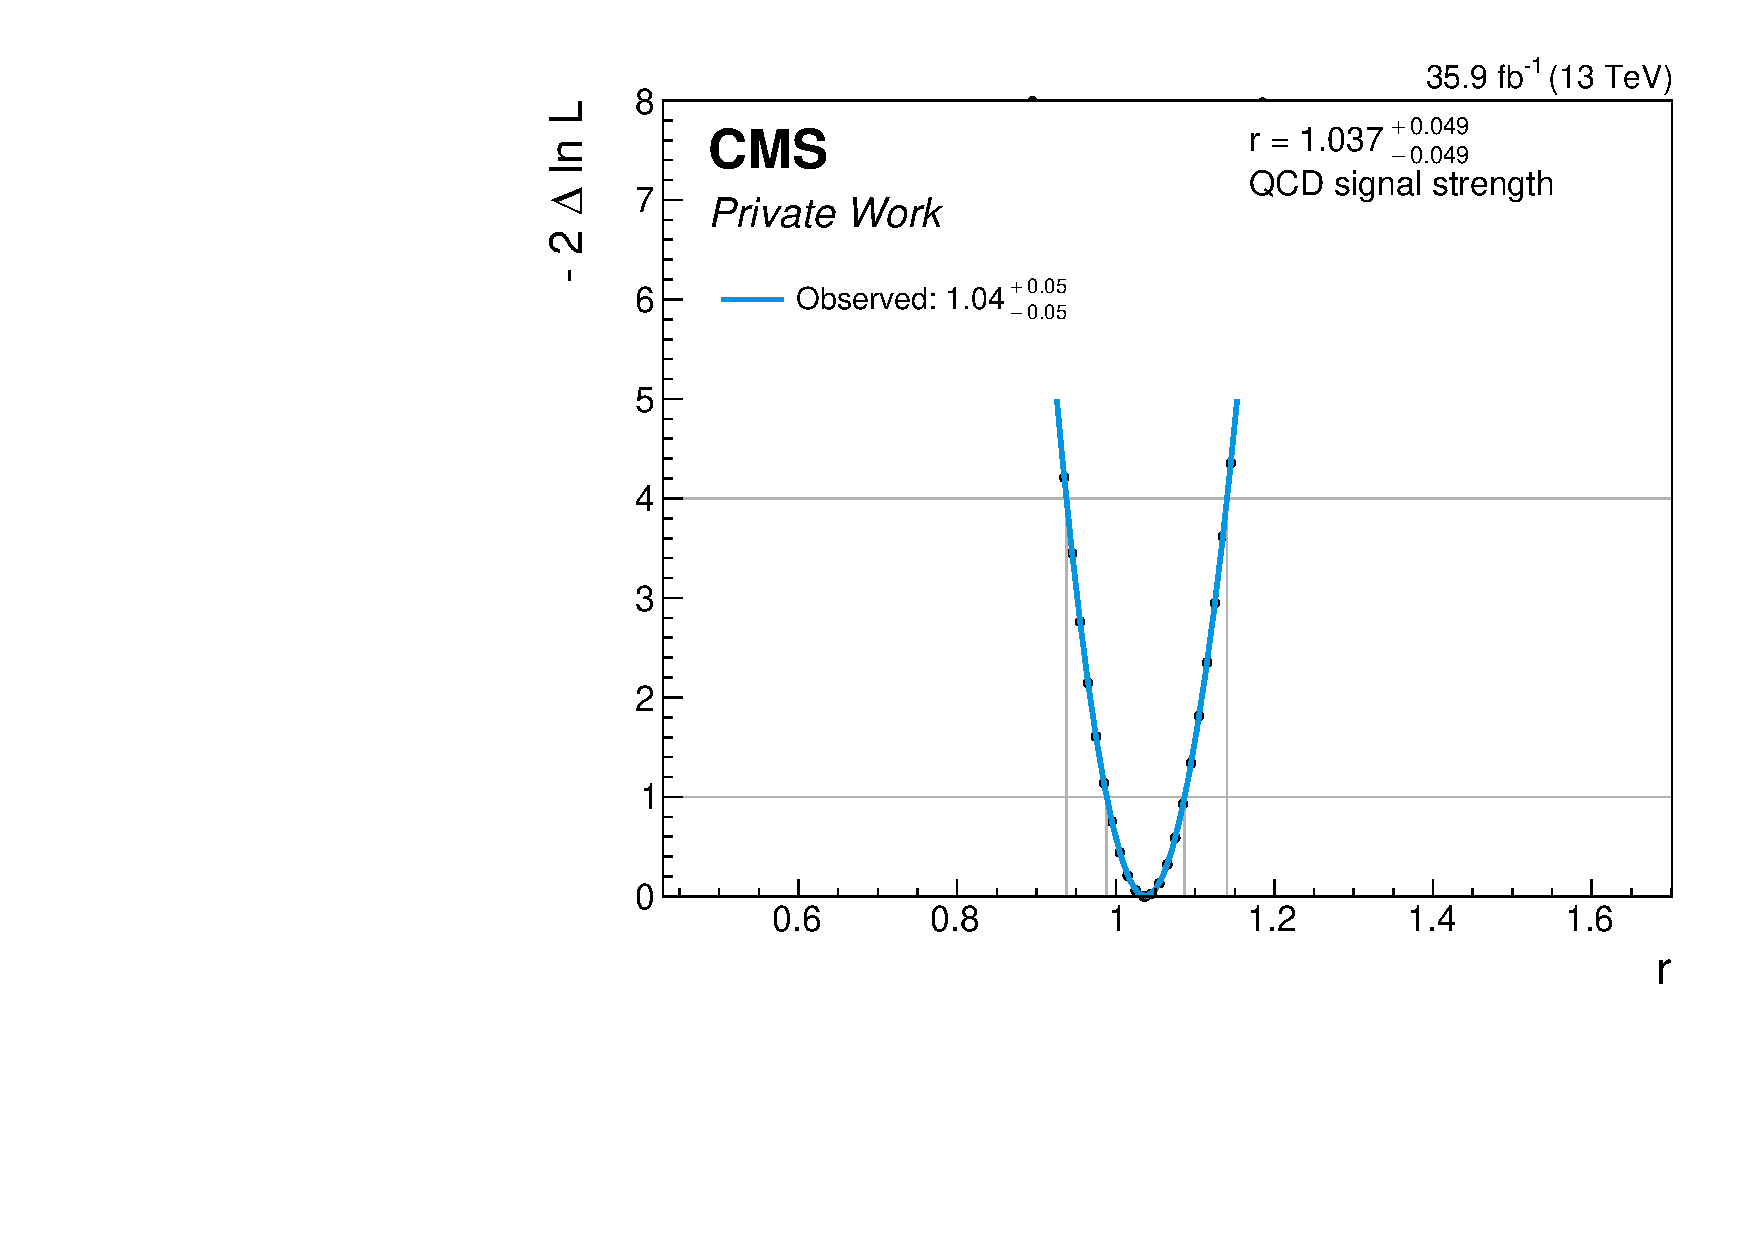
\includegraphics[width=.49\textwidth]{Figures/background_estimation/RQCDOSSS/Scans/et_ZeroJet2D_antiiso_far/plots/nll.pdf}
    \caption[Results of the maximum likelihood scan for $R_\text{QCD}^\text{OS/SS}$ in the \etau{} channel for the \textit{0-jet} category.]{Results of the maximum likelihood scan to find the signal strength of the QCD multijet background in the \etau channel in the \textit{boosted} category.
    The signal strength parameter from the near sideband (left figure) $r^{\text{near}}_\text{QCD} = 1.20\pm 0.08$ is taken as the QCD OS/SS factor. As statistical uncertainty the larger value of the two given thresholds is chosen. 
    $r^{\text{near}}_\text{QCD}$ is compared to the value $r^{\text{far}}_\text{QCD} = 1.04\pm 0.05$ obtained in the \textit{far} sideband (right plot). As they agree within their uncertainties the statistical uncertainties of the far sideband is assigned as systematic extrapolation uncertainty.}\label{SUPPLE:BK:Scans:et_0jet}
\end{figure}%
 

\begin{figure}[h!]
    \centering
    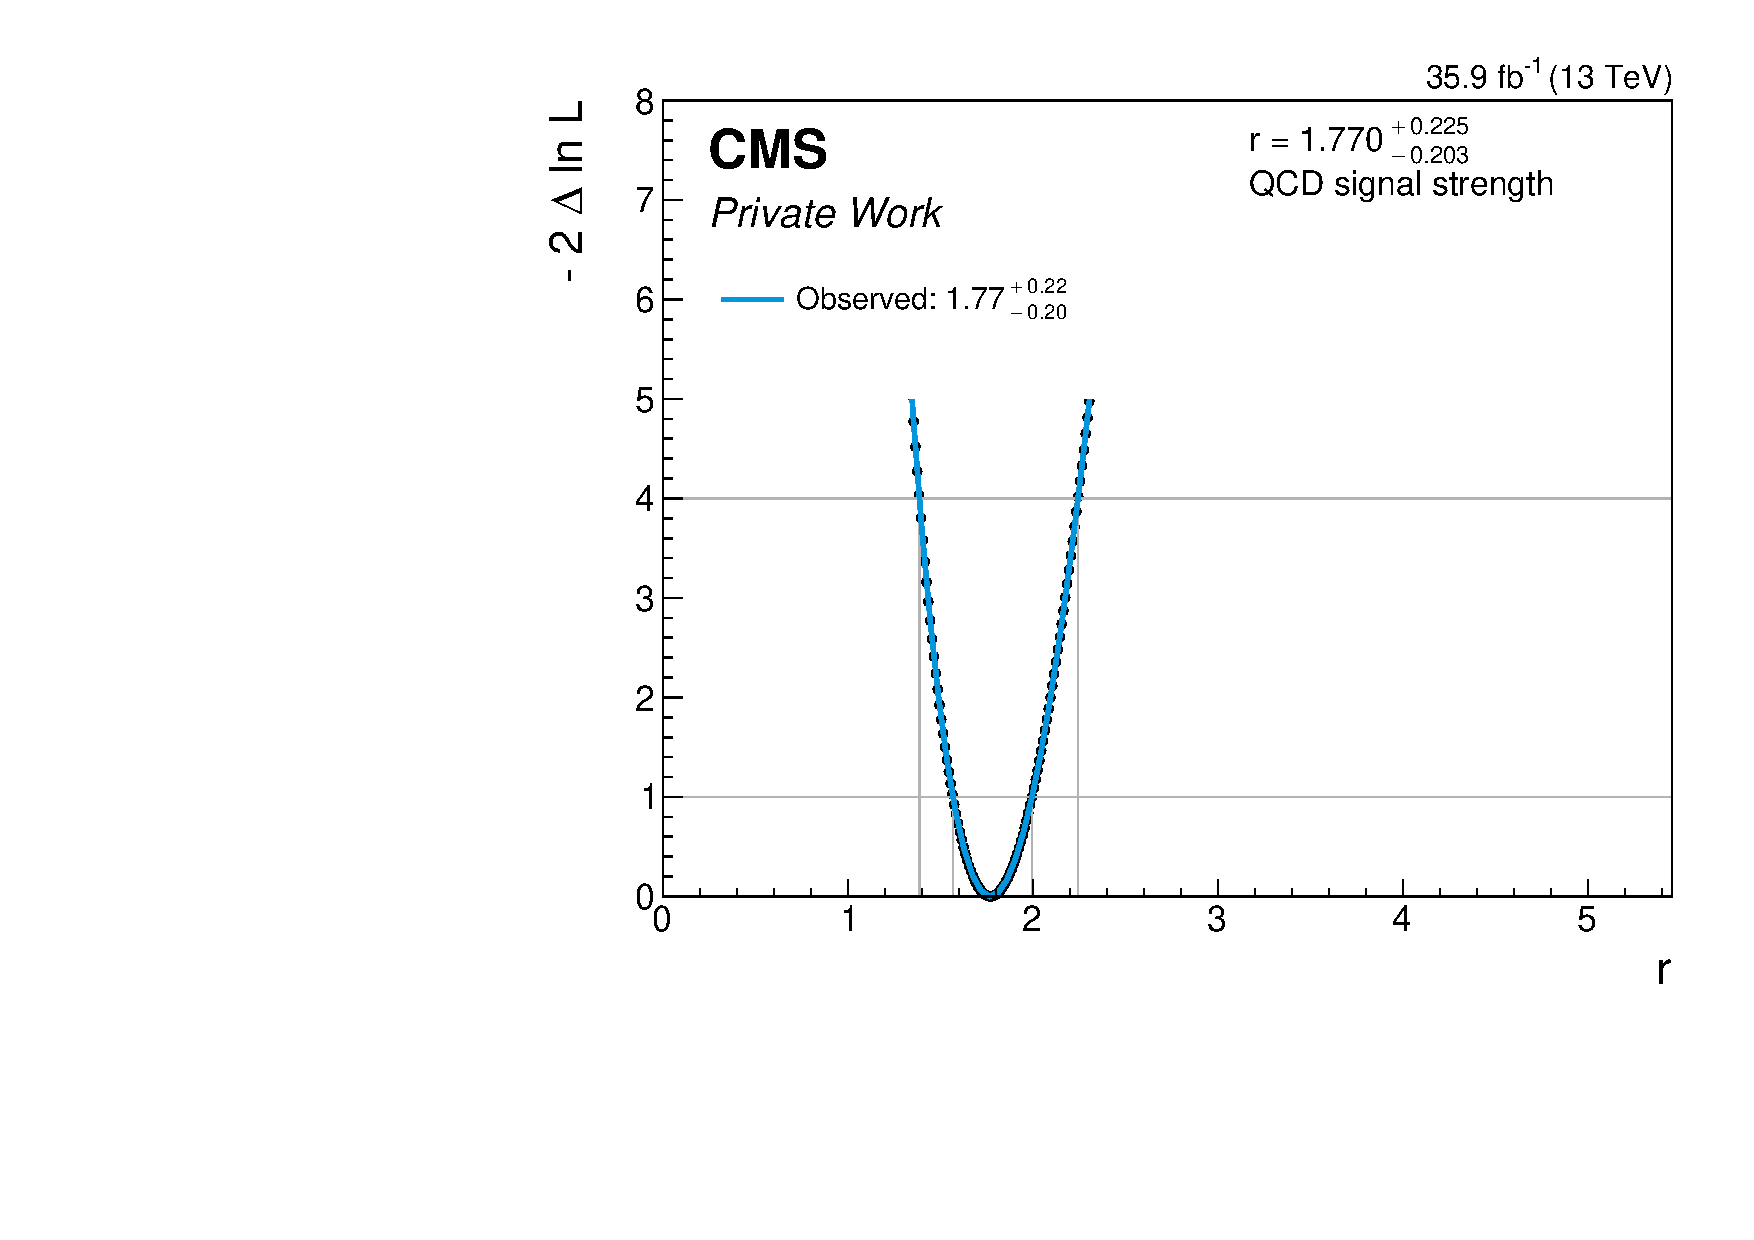
\includegraphics[width=.49\textwidth]{Figures/background_estimation/RQCDOSSS/Scans/et_Boosted2D_antiiso_near/plots/nll.pdf}
    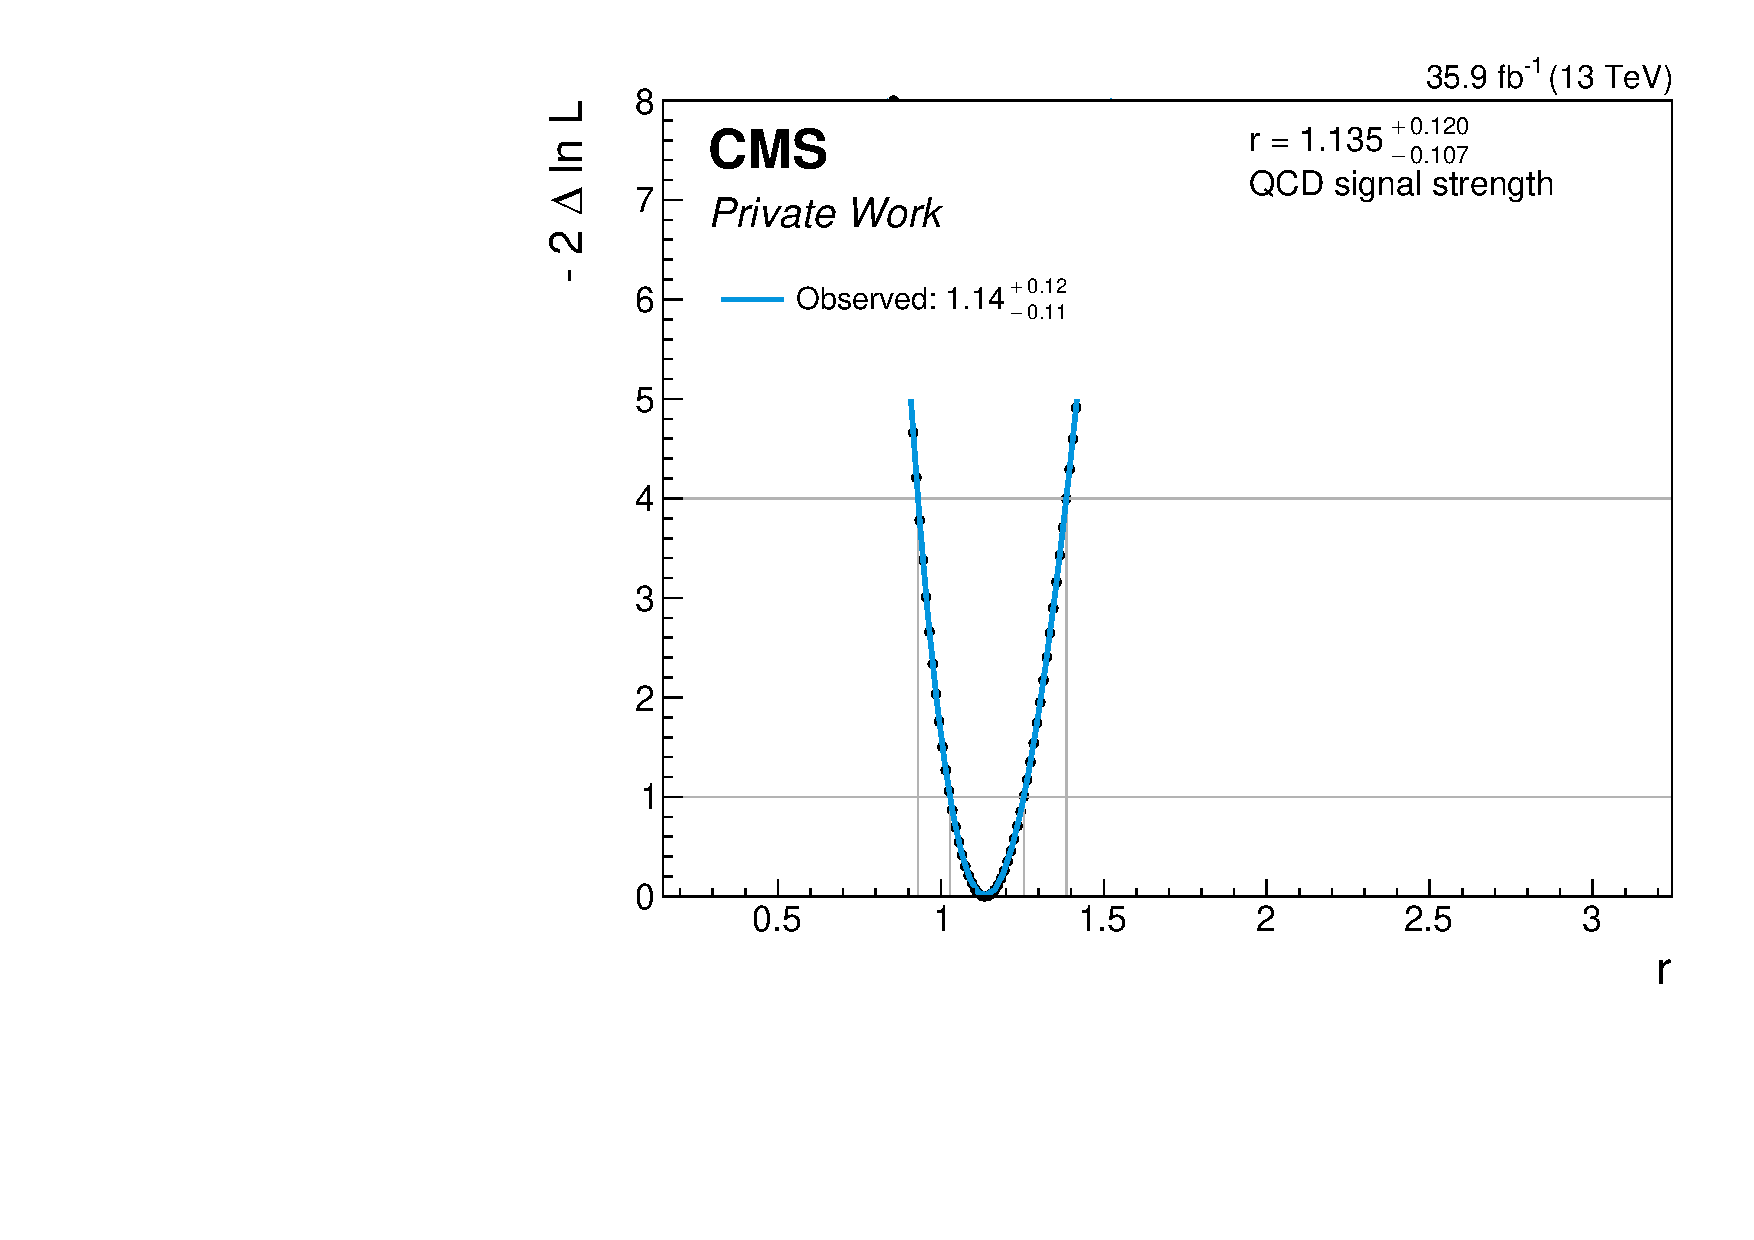
\includegraphics[width=.49\textwidth]{Figures/background_estimation/RQCDOSSS/Scans/et_Boosted2D_antiiso_far/plots/nll.pdf}
    \caption[Results of the maximum likelihood scan for $R_\text{QCD}^\text{OS/SS}$ in the \etau{} channel for the \textit{boosted} category.]{Results of the maximum likelihood scan to find the signal strength of the QCD multijet background in the \etau channel in the \textit{boosted} category.
    The signal strength parameter from the near sideband (left figure) $r^{\text{near}}_\text{QCD} = 1.77\pm 0.23$ is taken as the QCD OS/SS factor. As statistical uncertainty the larger value of the two given thresholds is chosen. 
    $r^{\text{near}}_\text{QCD}$ is compared to the value $r^{\text{far}}_\text{QCD} = 1.13\pm 0.12$ obtained in the \textit{far} sideband (right plot). As they agree within their uncertainties the statistical uncertainties of the far sideband is assigned as systematic extrapolation uncertainty.}\label{SUPPLE:BK:Scans:et_boosted}
\end{figure}

\begin{figure}[h!]
    \centering
    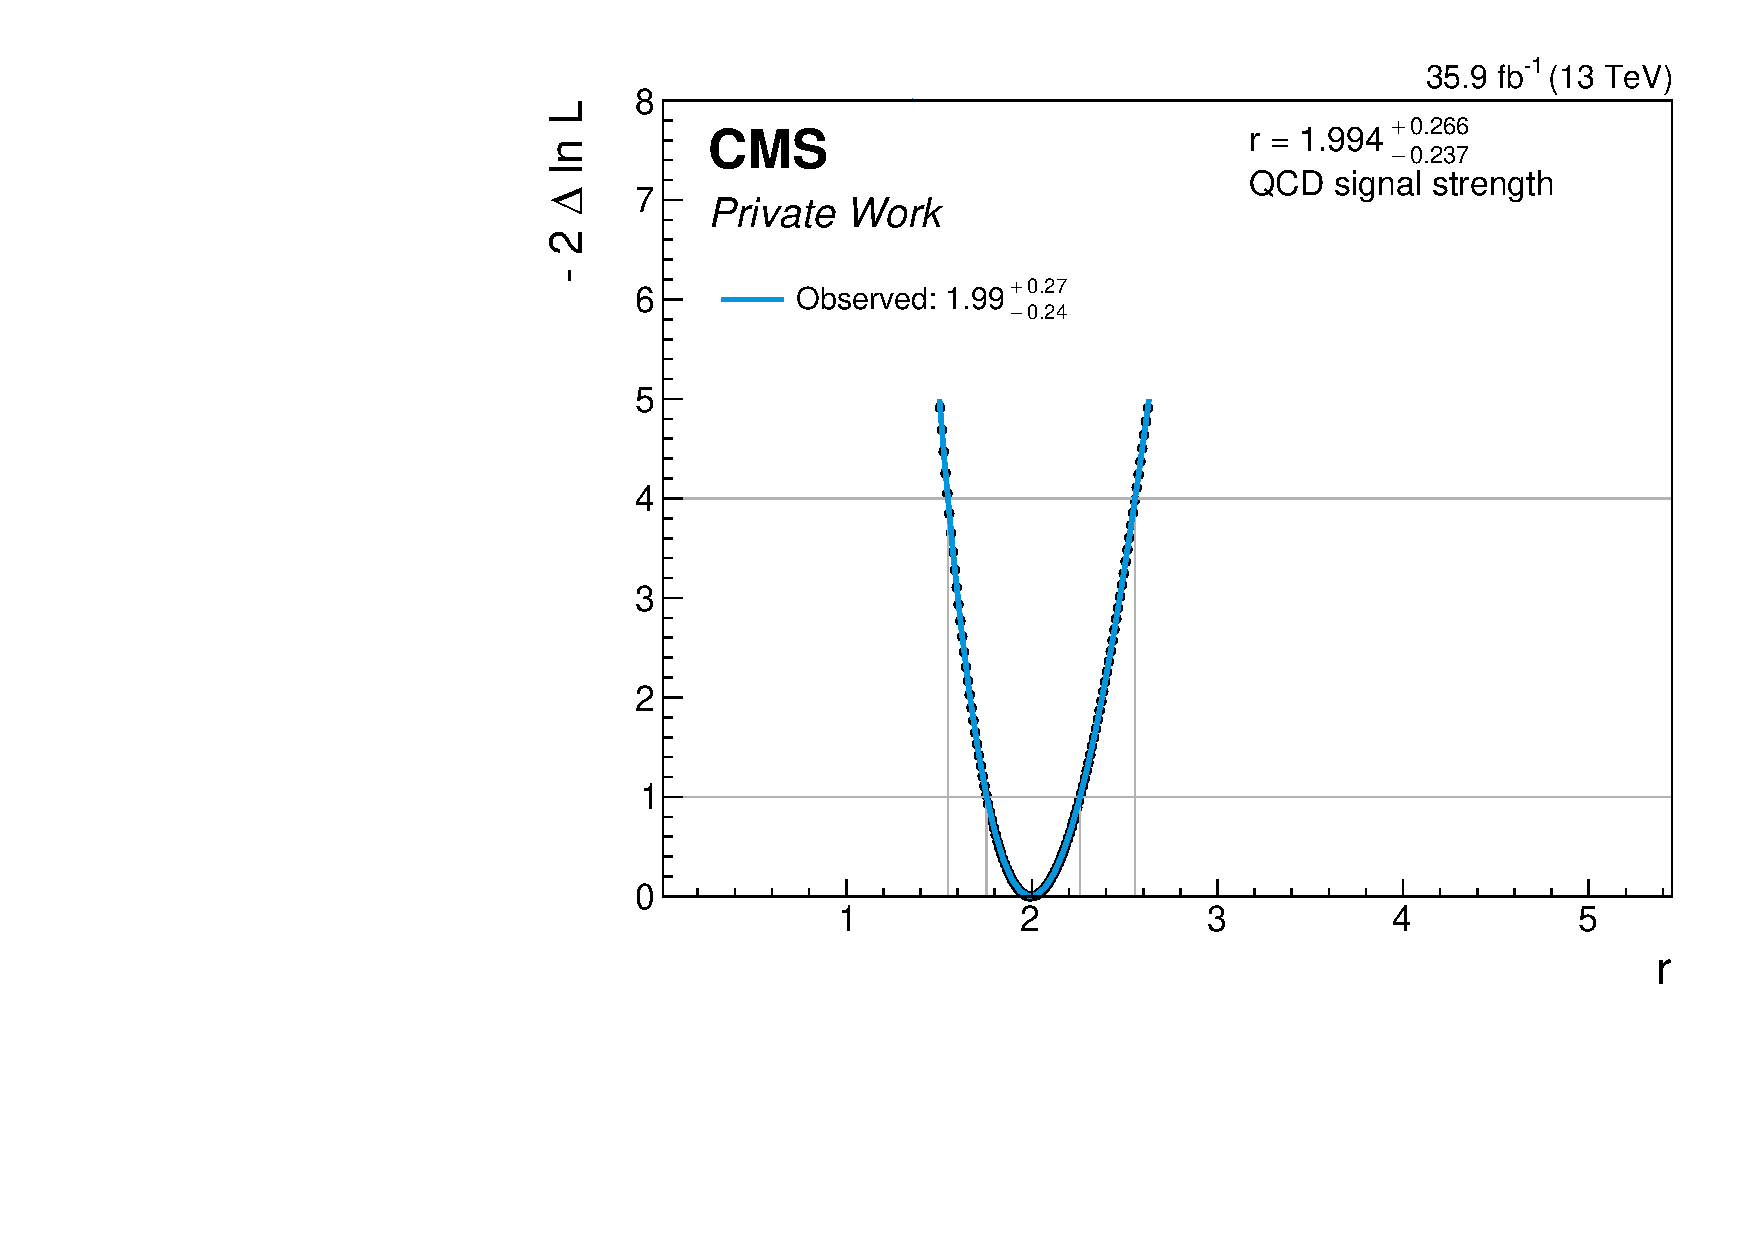
\includegraphics[width=.49\textwidth]{Figures/background_estimation/RQCDOSSS/Scans/et_dijet2D_antiiso_near/plots/nll.pdf}
    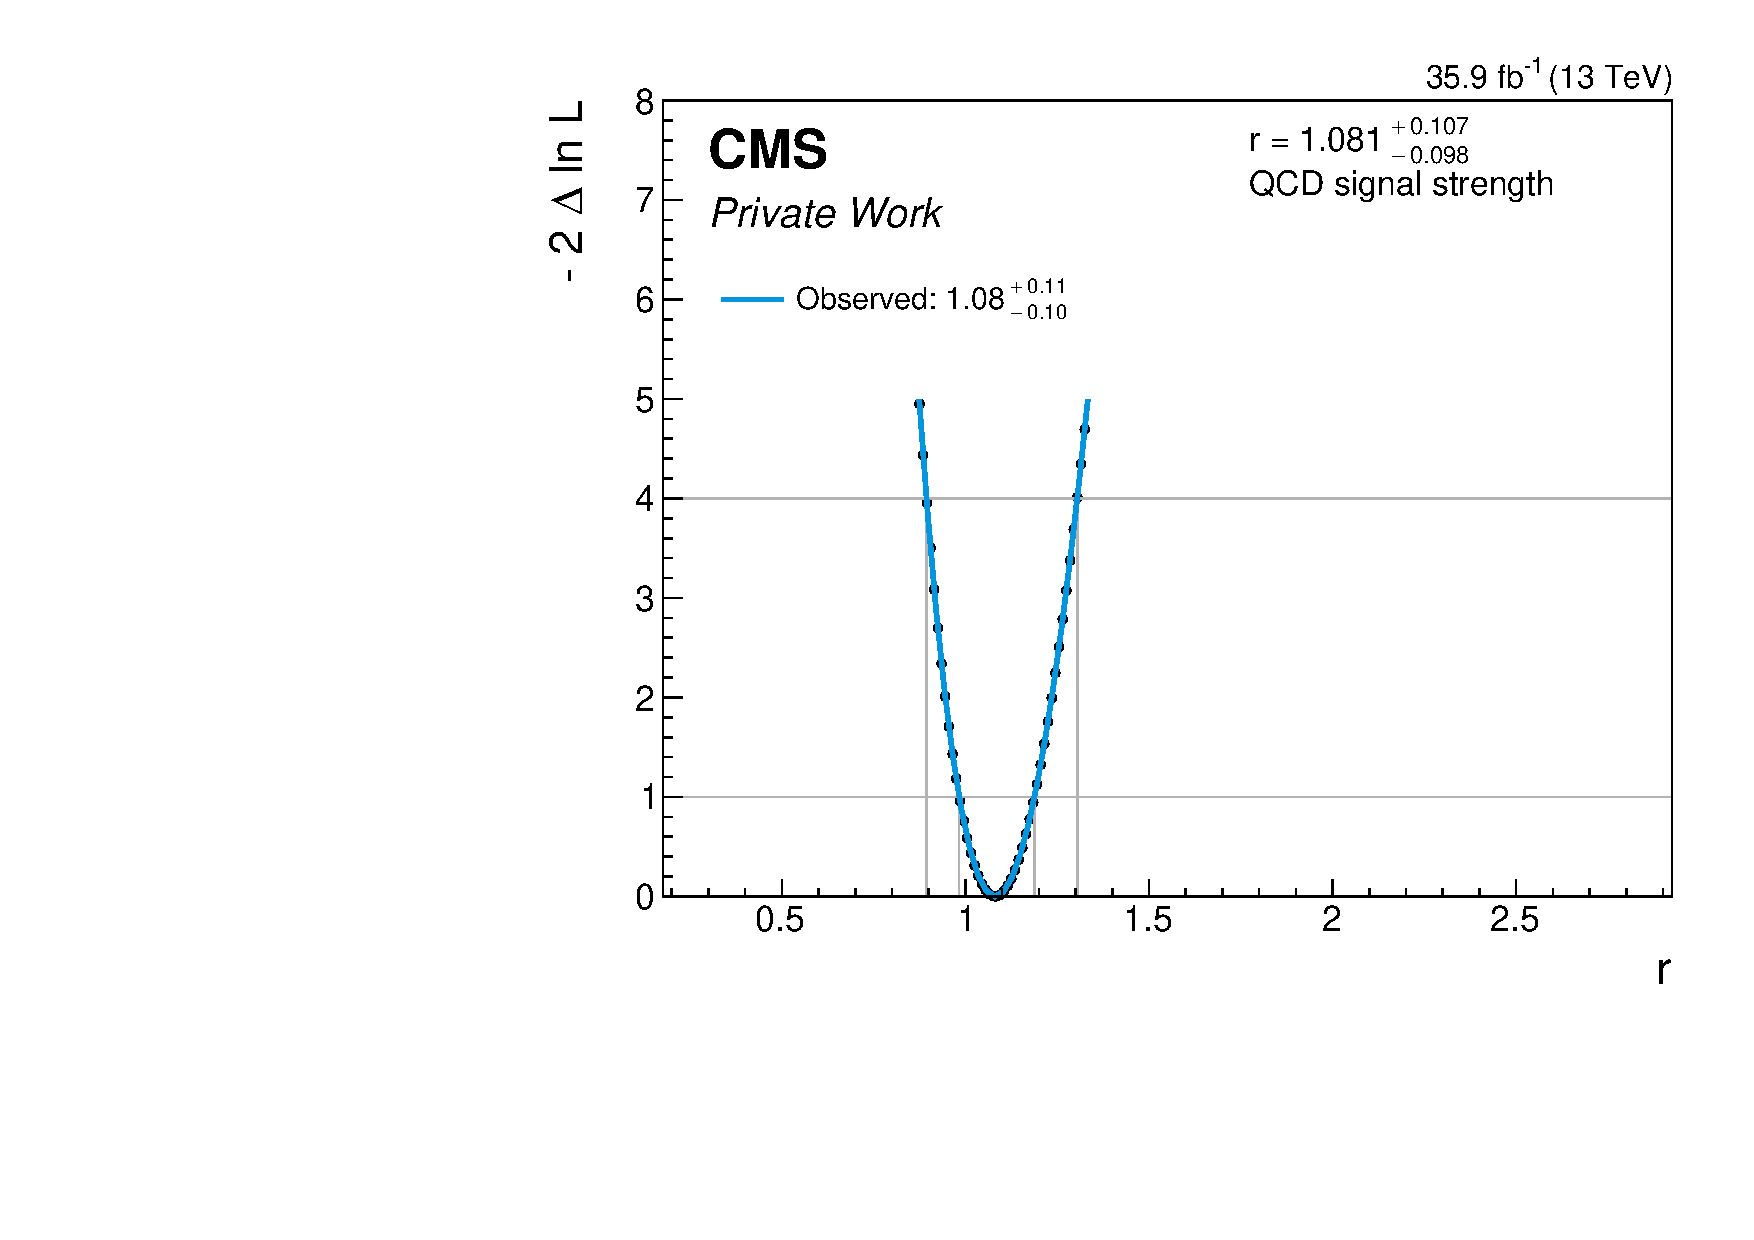
\includegraphics[width=.49\textwidth]{Figures/background_estimation/RQCDOSSS/Scans/et_dijet2D_antiiso_far/plots/nll.pdf}
    \caption[Results of the maximum likelihood scan for $R_\text{QCD}^\text{OS/SS}$ in the \etau{} channel for the \textit{dijet} category.]{Results of the maximum likelihood scan to find the signal strength of the QCD multijet background in the \etau channel in the \textit{boosted} category.
    The signal strength parameter from the near sideband (left figure) $r^{\text{near}}_\text{QCD} = 2.00\pm 0.27$ is taken as the QCD OS/SS factor. As statistical uncertainty the larger value of the two given thresholds is chosen. 
    $r^{\text{near}}_\text{QCD}$ is compared to the value $r^{\text{far}}_\text{QCD} = 1.08\pm 0.1$ obtained in the \textit{far} sideband (right plot). As they agree within their uncertainties the statistical uncertainties of the far sideband is assigned as systematic extrapolation uncertainty.}\label{SUPPLE:BK:Scans:et_2jet}
\end{figure}

\subsubsection{\mutau{} channel}

\begin{figure}[h!]
    \centering
    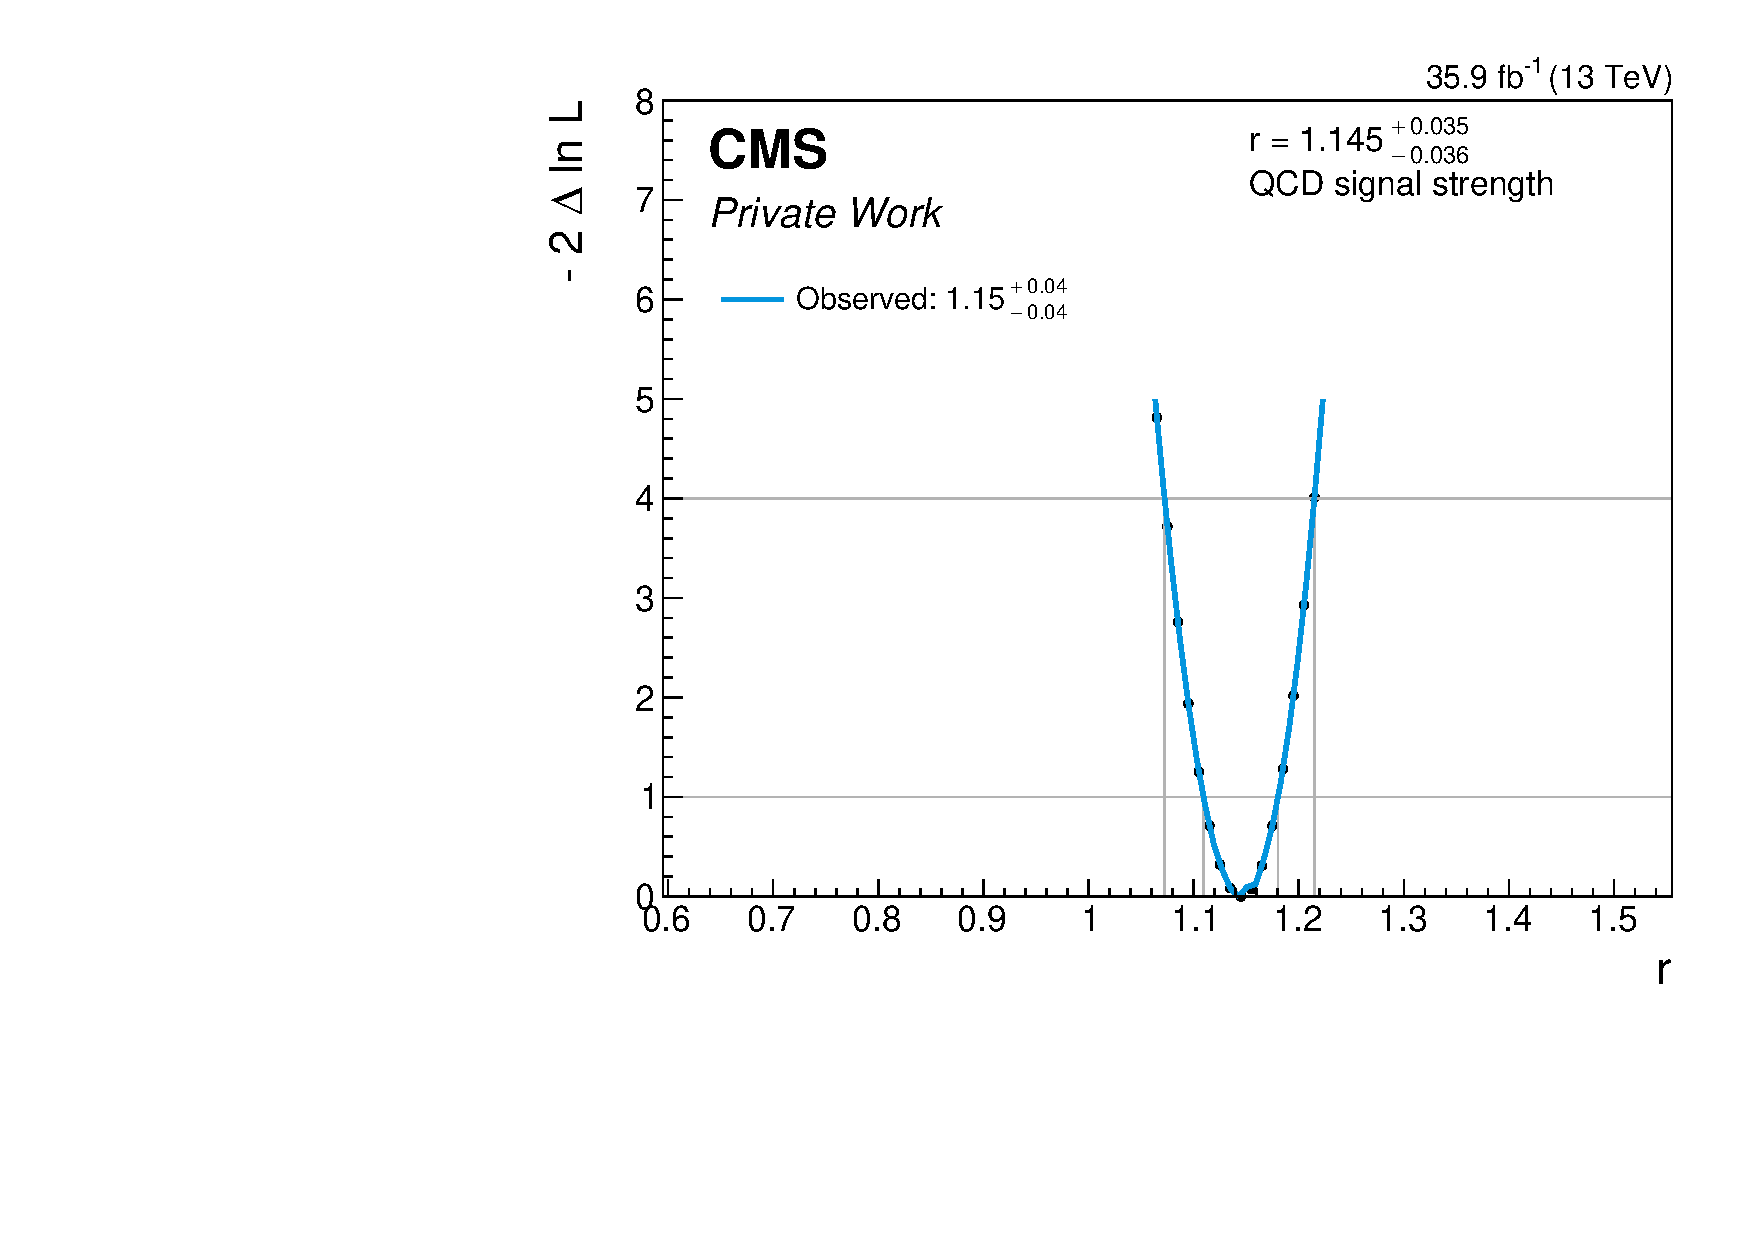
\includegraphics[width=.49\textwidth]{Figures/background_estimation/RQCDOSSS/Scans/mt_ZeroJet2D_antiiso_near/plots/nll.pdf}
    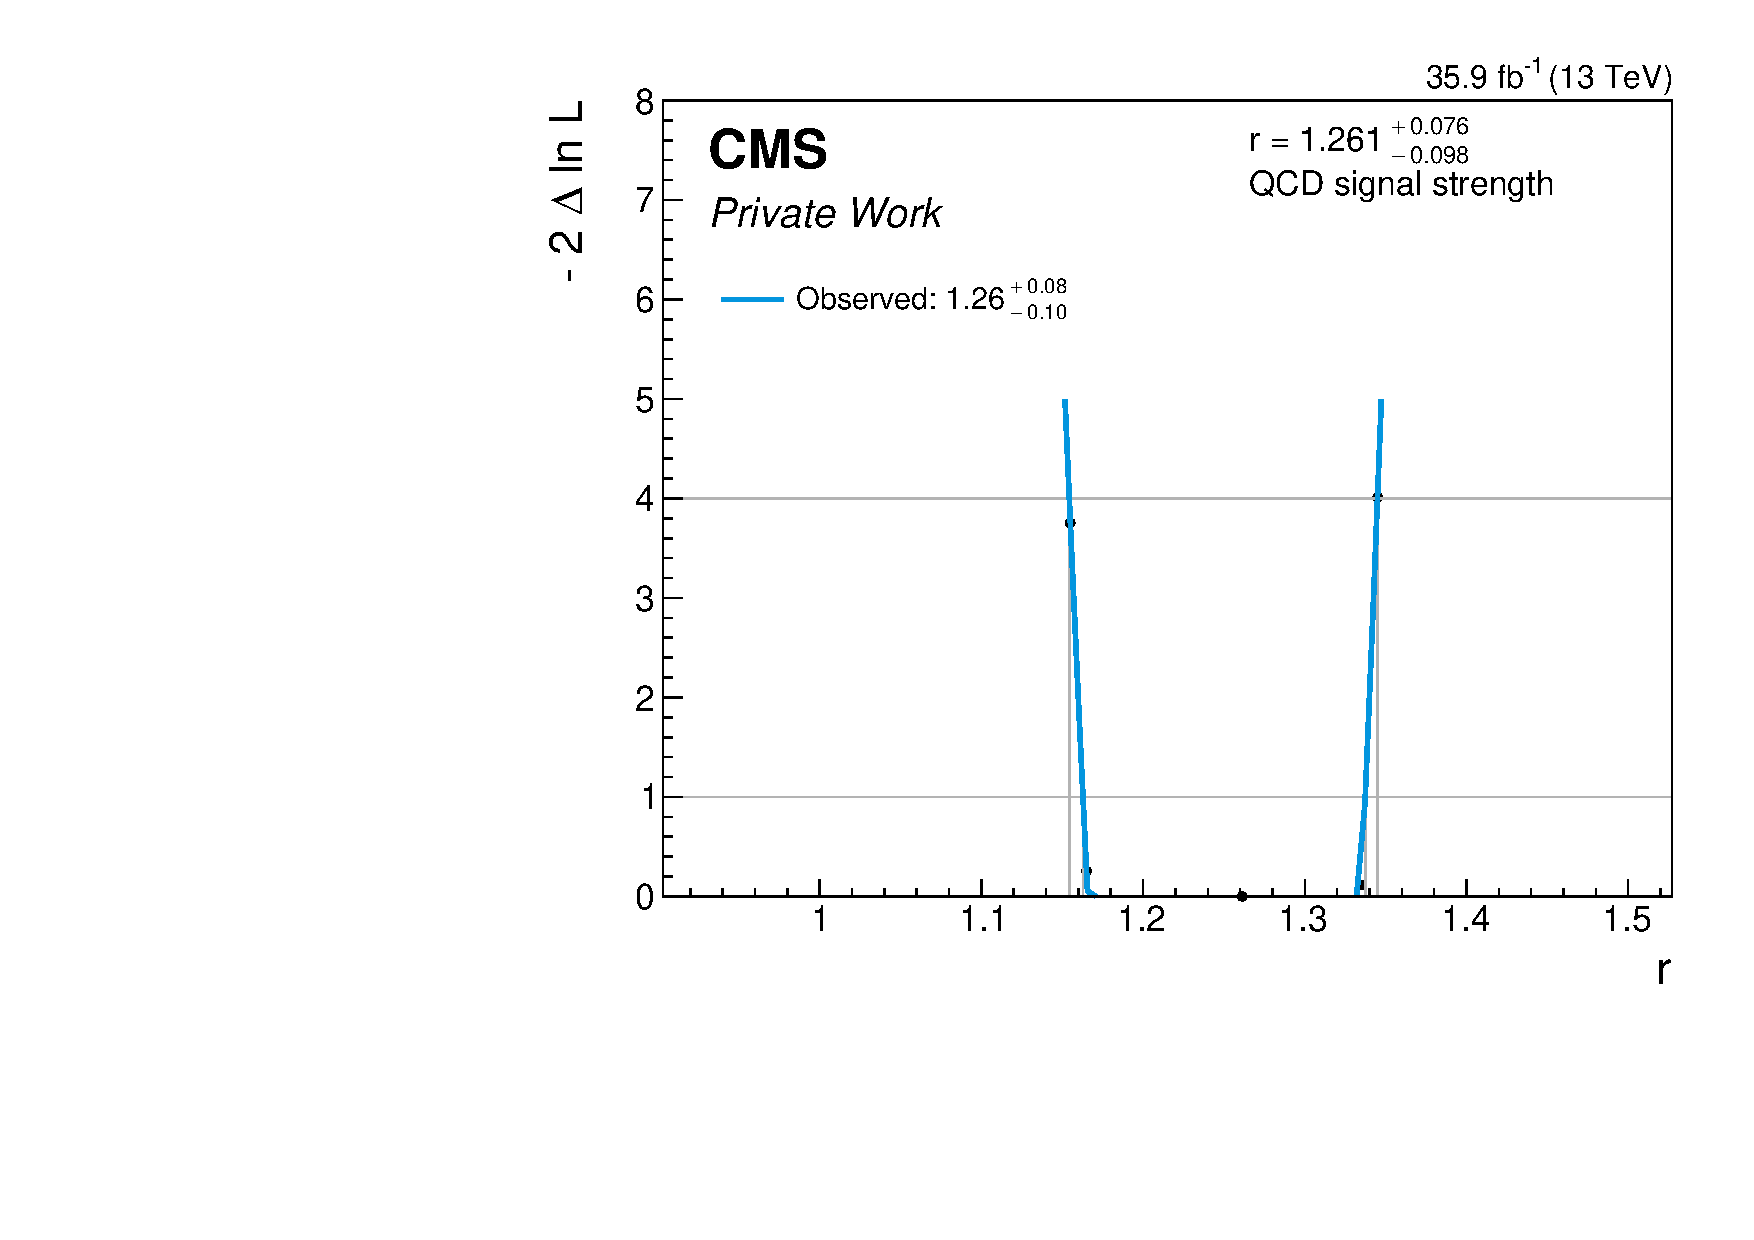
\includegraphics[width=.49\textwidth]{Figures/background_estimation/RQCDOSSS/Scans/mt_ZeroJet2D_antiiso_far/plots/nll.pdf}
    \caption[Results of the maximum likelihood scan for $R_\text{QCD}^\text{OS/SS}$ in the \mutau{} channel for the \textit{0-jet} category.]{Results of the maximum likelihood scan to find the signal strength of the QCD multijet background in the \mutau{} channel in the \textit{boosted} category.
    The signal strength parameter from the near sideband (left figure) $r^{\text{near}}_\text{QCD} = 1.19\pm 0.06$ is taken as the QCD OS/SS factor. As statistical uncertainty the larger value of the two given thresholds is chosen. 
    $r^{\text{near}}_\text{QCD}$ is compared to the value $r^{\text{far}}_\text{QCD} = 1.26\pm 0.10$ obtained in the \textit{far} sideband (right plot). As they agree within their uncertainties the statistical uncertainties of the far sideband is assigned as systematic extrapolation uncertainty.}\label{SUPPLE:BK:Scans:mt_0jet}
\end{figure}


\begin{figure}[h!]
    \centering
    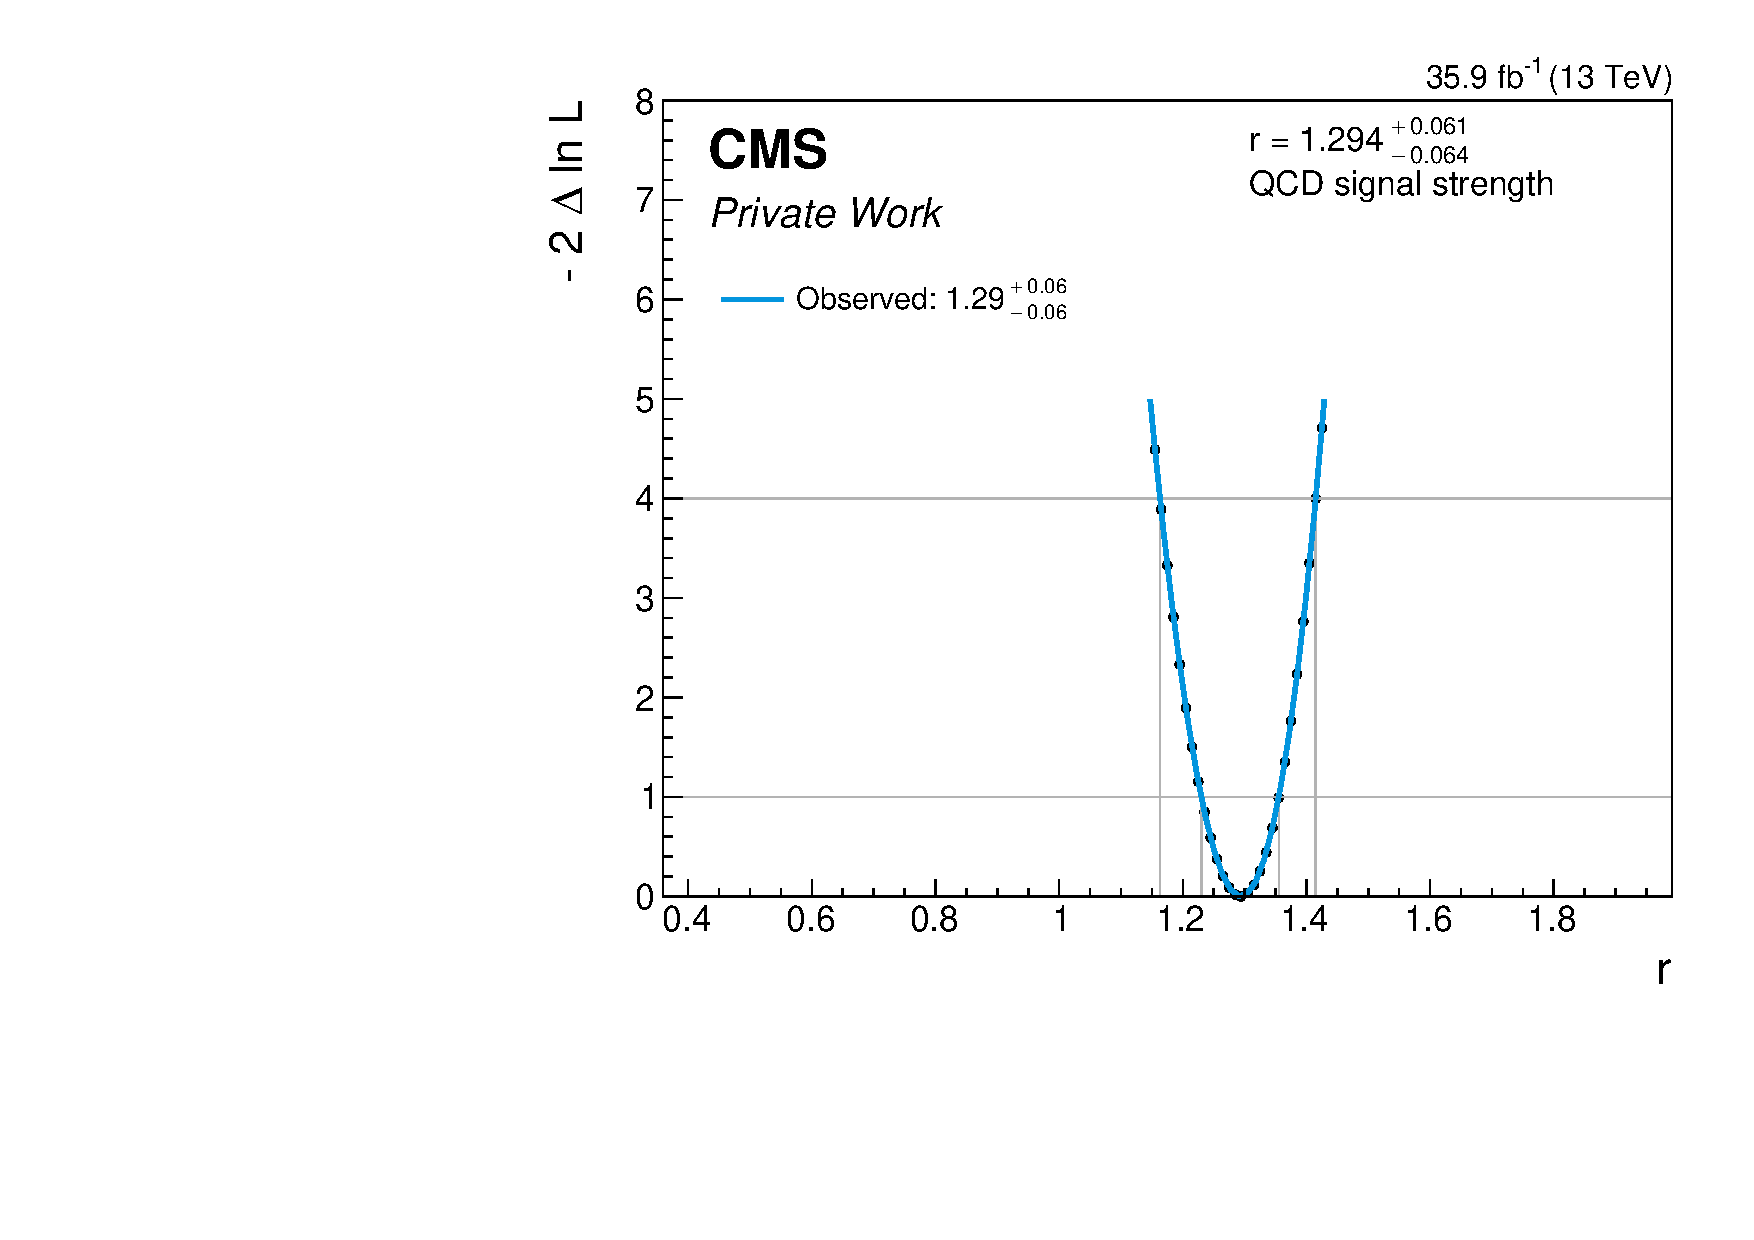
\includegraphics[width=.49\textwidth]{Figures/background_estimation/RQCDOSSS/Scans/mt_dijet2D_antiiso_near/plots/nll.pdf}
    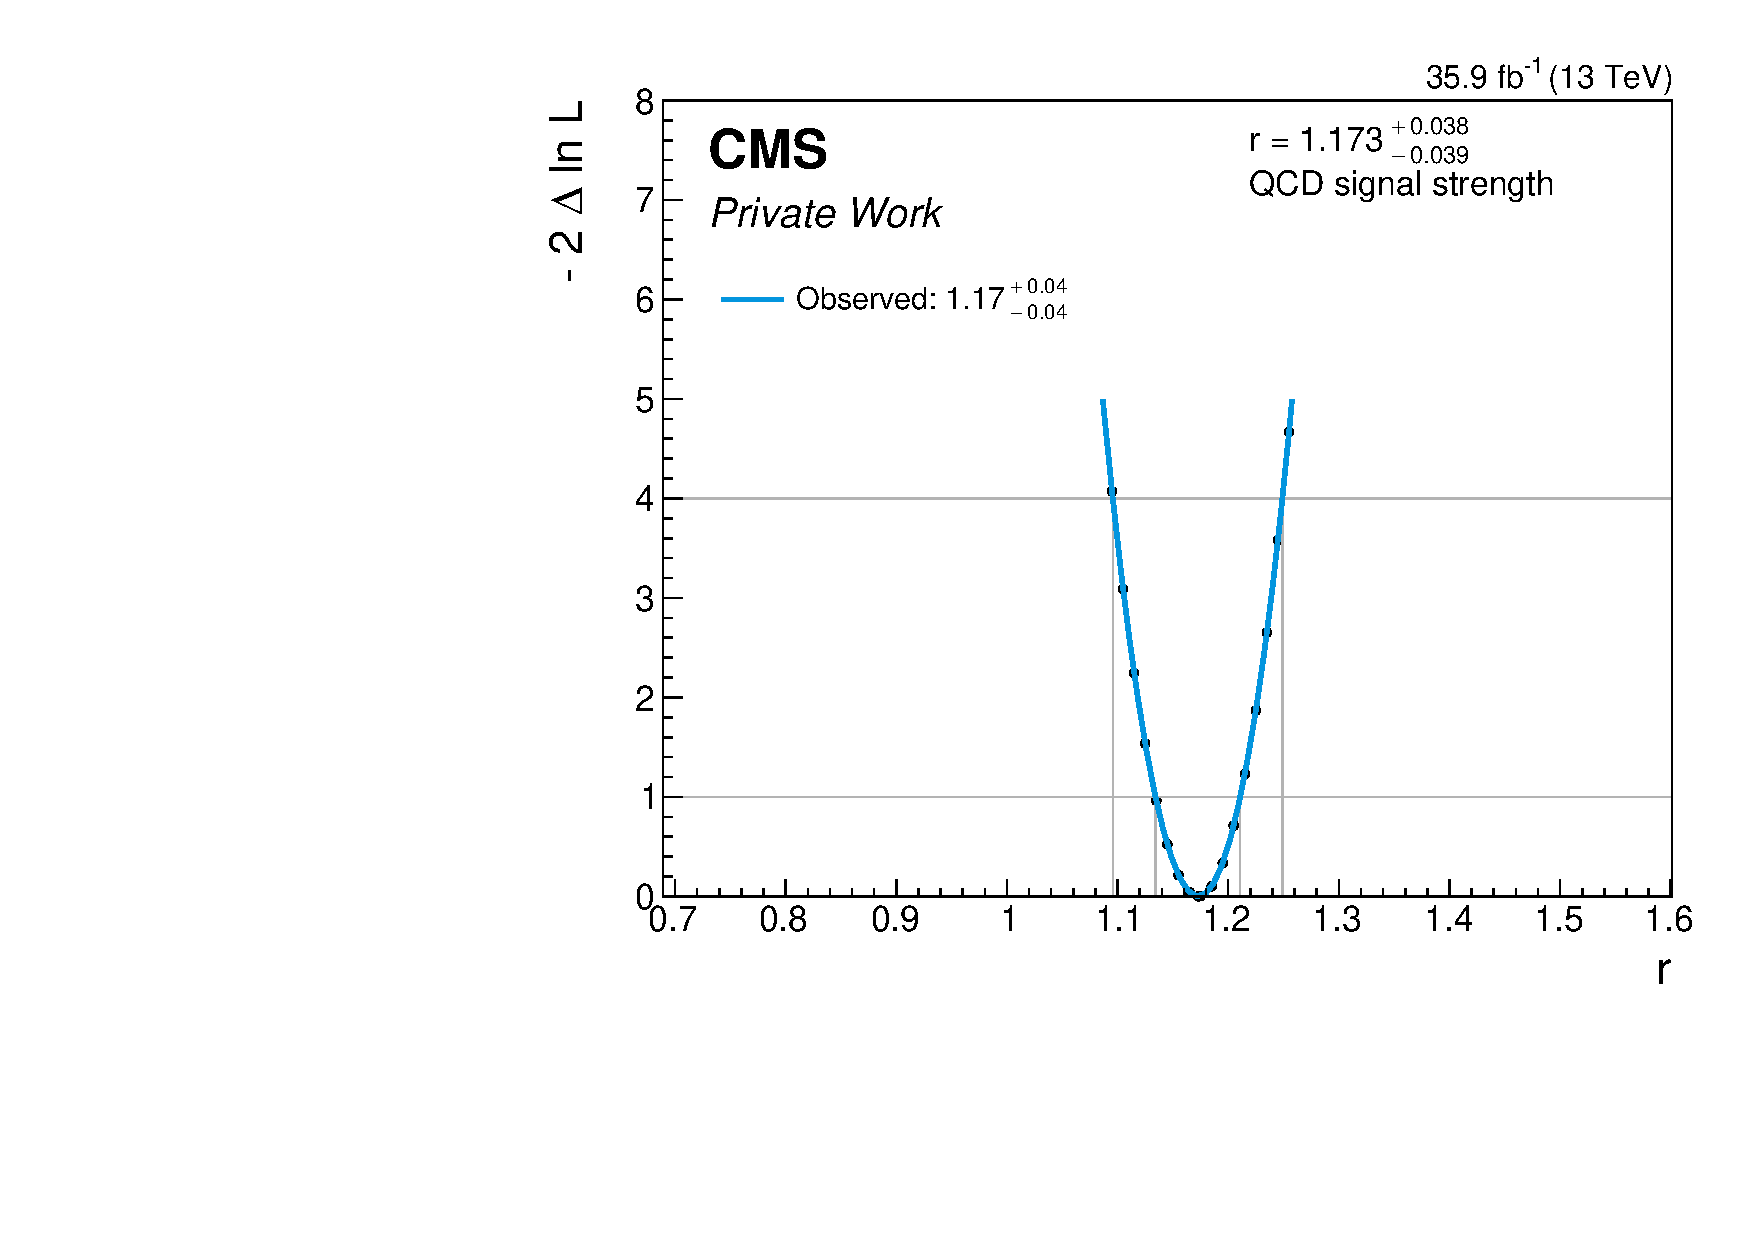
\includegraphics[width=.49\textwidth]{Figures/background_estimation/RQCDOSSS/Scans/mt_dijet2D_antiiso_far/plots/nll.pdf}
    \caption[Results of the maximum likelihood scan for $R_\text{QCD}^\text{OS/SS}$ in the \mutau{} channel for the \textit{dijet} category.]{Results of the maximum likelihood scan to find the signal strength of the QCD multijet background in the \mutau{} channel in the \textit{boosted} category.
    The signal strength parameter from the near sideband (left figure) $r^{\text{near}}_\text{QCD} = 1.29\pm  0.6$ is taken as the QCD OS/SS factor. As statistical uncertainty the larger value of the two given thresholds is chosen. 
    $r^{\text{near}}_\text{QCD}$ is compared to the value $r^{\text{far}}_\text{QCD} = 1.17\pm 0.04$ obtained in the \textit{far} sideband (right plot). As they agree within their uncertainties the statistical uncertainties of the far sideband is assigned as systematic extrapolation uncertainty.}\label{SUPPLE:BK:Scans:mt_2jet}
\end{figure}

\begin{figure}[h!]
    \centering
    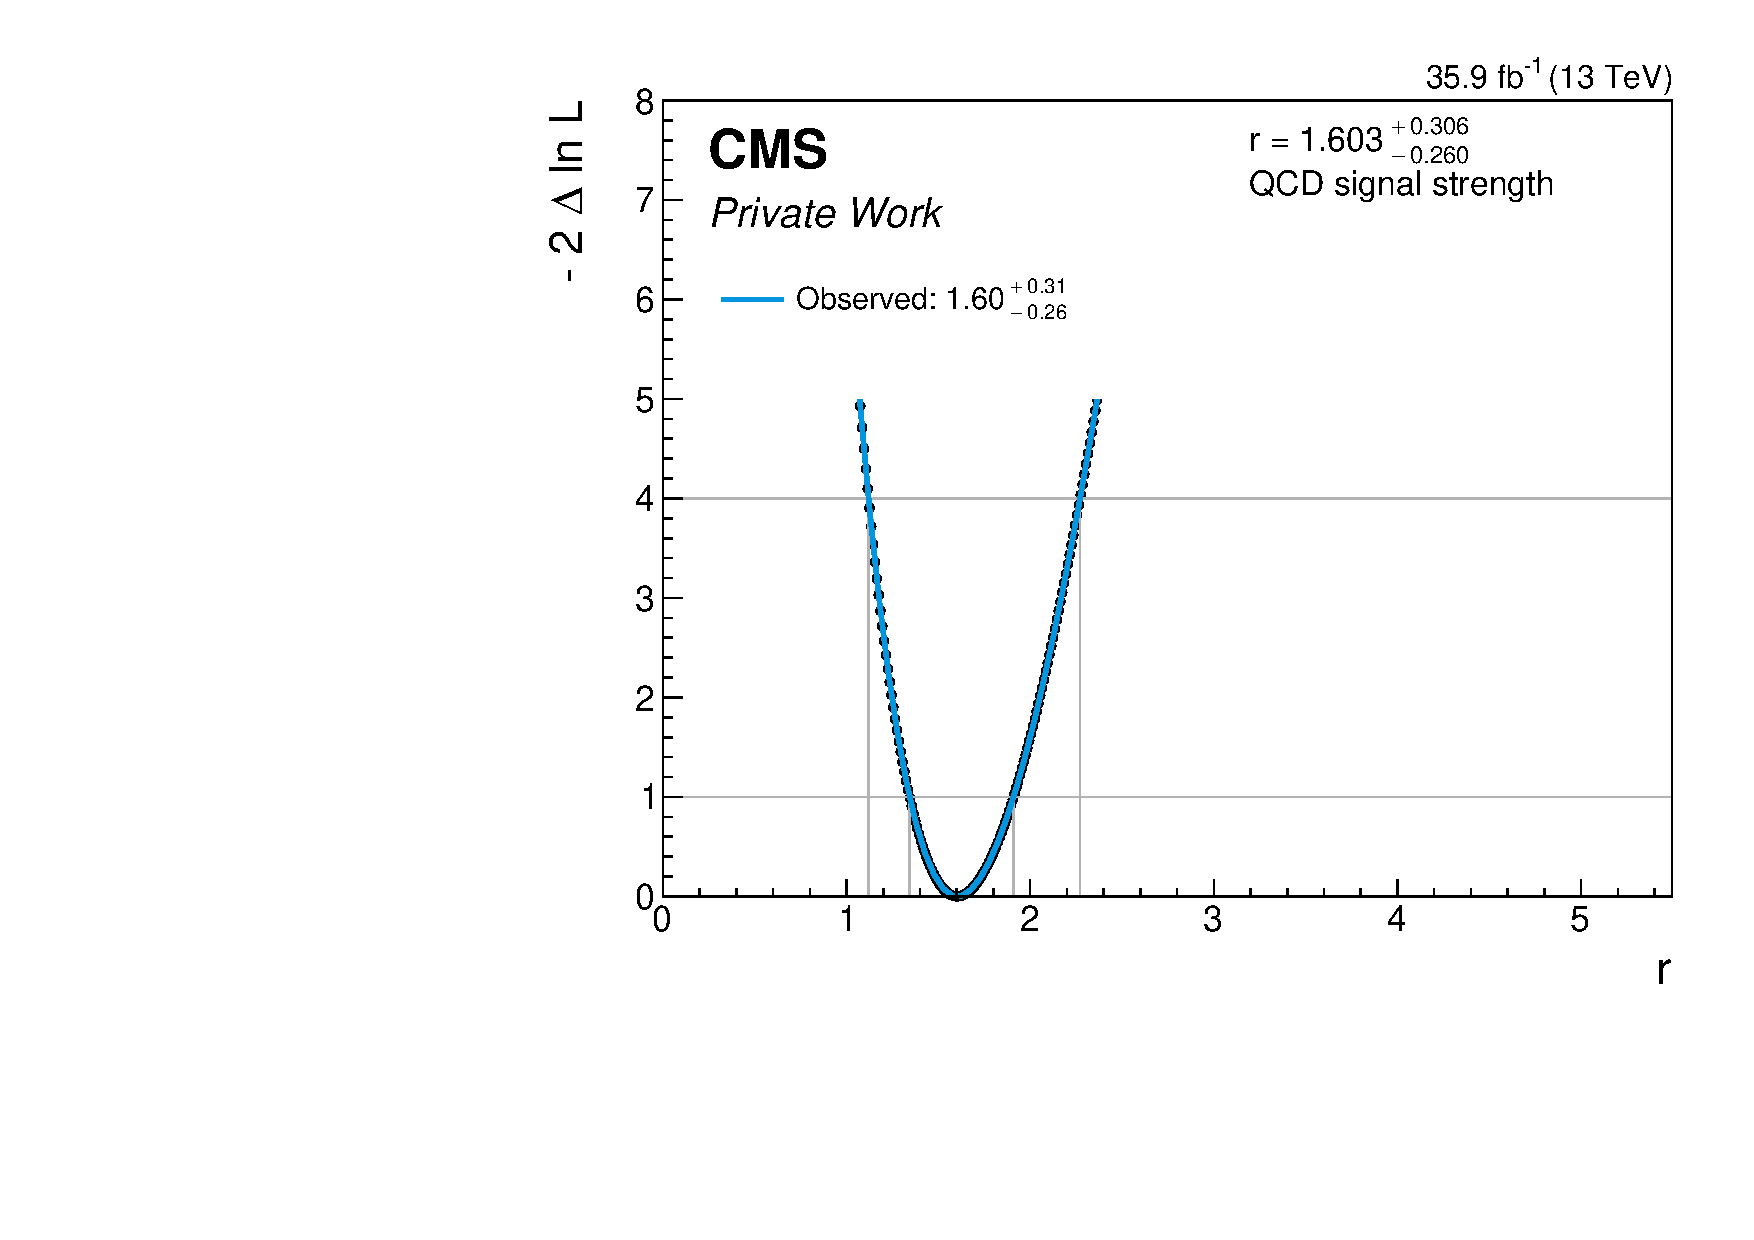
\includegraphics[width=.49\textwidth]{Figures/background_estimation/RQCDOSSS/Scans/mt_dijet2D_lowboost_antiiso_near/nll.pdf}
    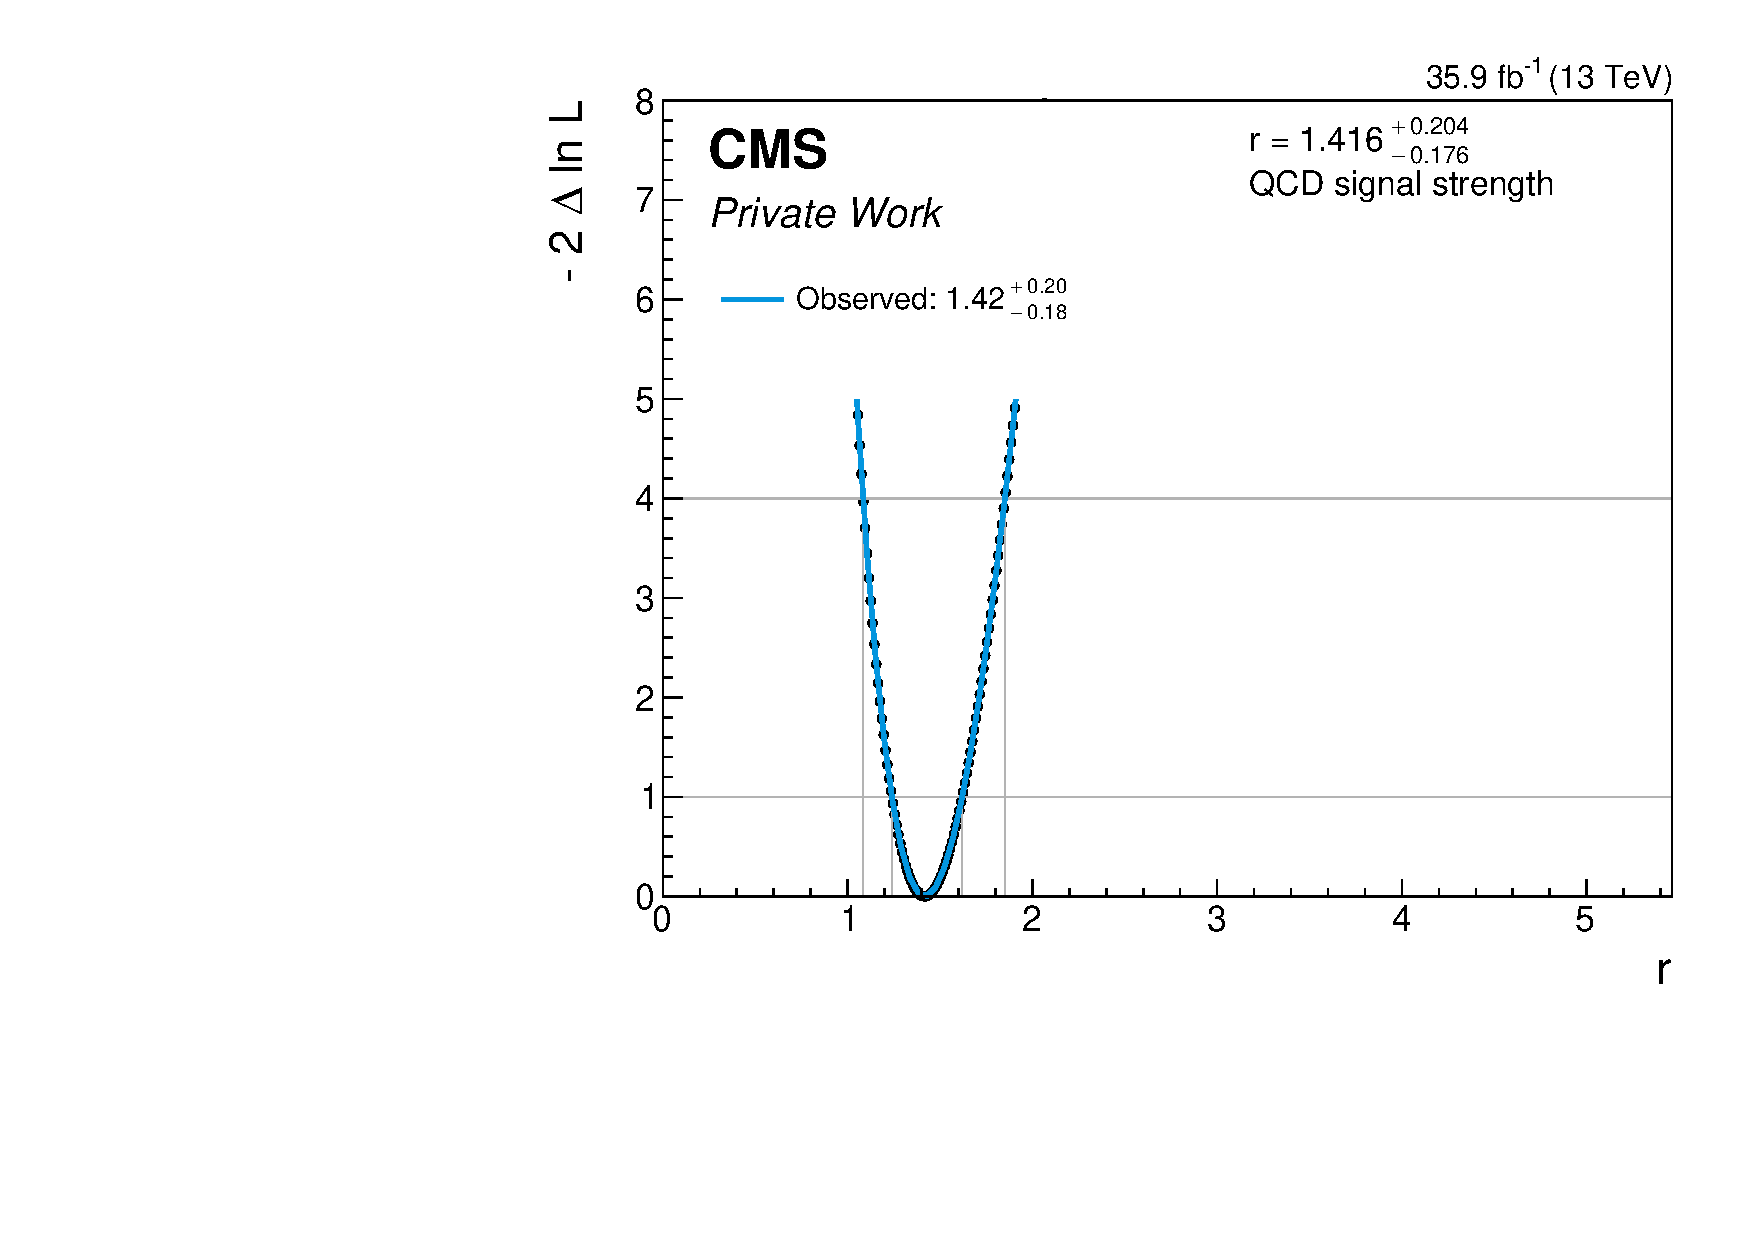
\includegraphics[width=.49\textwidth]{Figures/background_estimation/RQCDOSSS/Scans/mt_dijet2D_lowboost_antiiso_far/nll.pdf}
    \caption[Results of the maximum likelihood scan for $R_\text{QCD}^\text{OS/SS}$ in the \mutau{} channel for the \textit{dijet lowboost} category.]{Results of the maximum likelihood scan to find the signal strength of the QCD multijet background in the \mutau{} channel in the \textit{boosted} category.
    The signal strength parameter from the near sideband (left figure) $r^{\text{near}}_\text{QCD} = 1.60 \pm 0.3$ is taken as the QCD OS/SS factor. As statistical uncertainty the larger value of the two given thresholds is chosen. 
    $r^{\text{near}}_\text{QCD}$ is compared to the value $r^{\text{far}}_\text{QCD} = 1.42\pm 0.2$ obtained in the \textit{far} sideband (right plot). As they agree within their uncertainties the statistical uncertainties of the far sideband is assigned as systematic extrapolation uncertainty.}\label{SUPPLE:BK:Scans:mt_2jet}
\end{figure}
\clearpage
\subsection{QCD control regions}

\begin{figure}[h!]
     \centering
     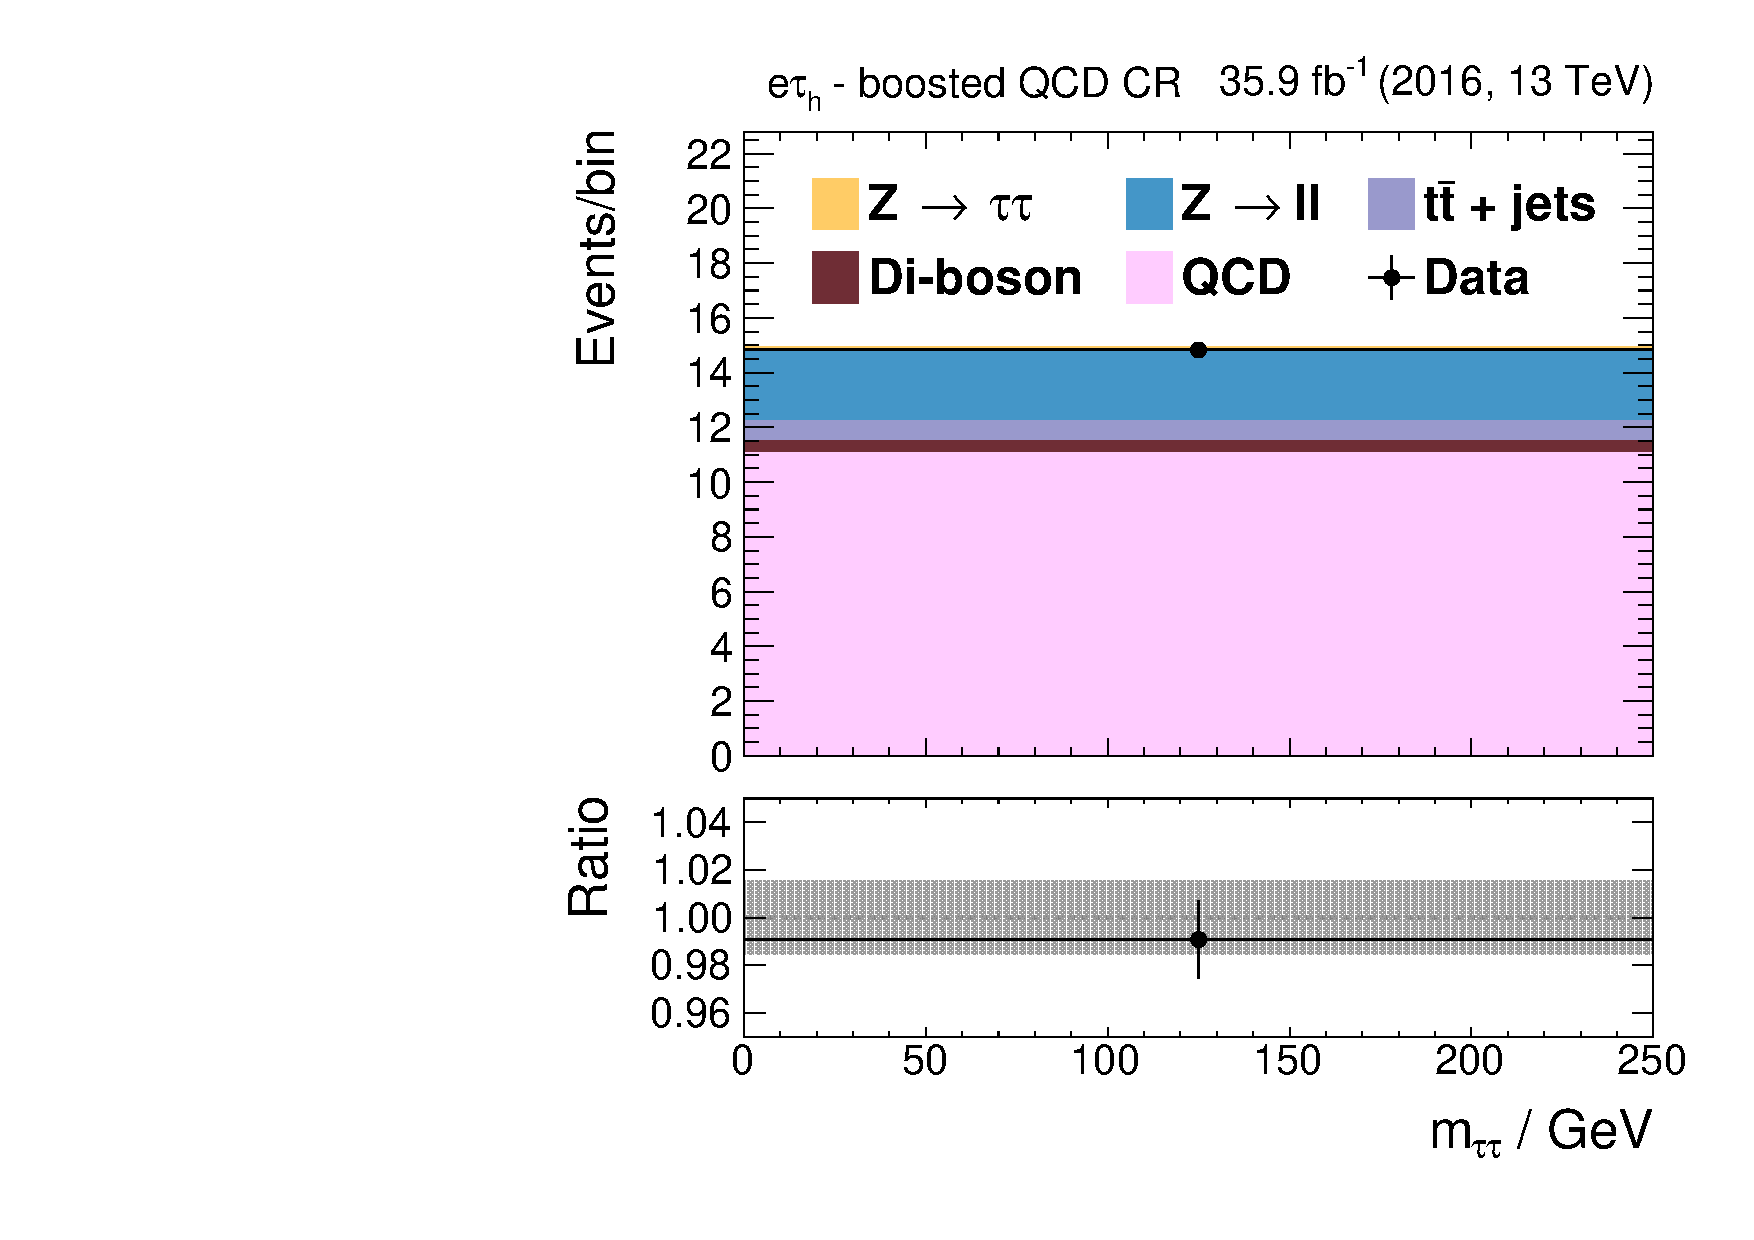
\includegraphics[width=0.47\textwidth]{Figures/background_estimation/qcd_et_control-regions/htt_inputet14__htt_et_14_13TeV.pdf}
     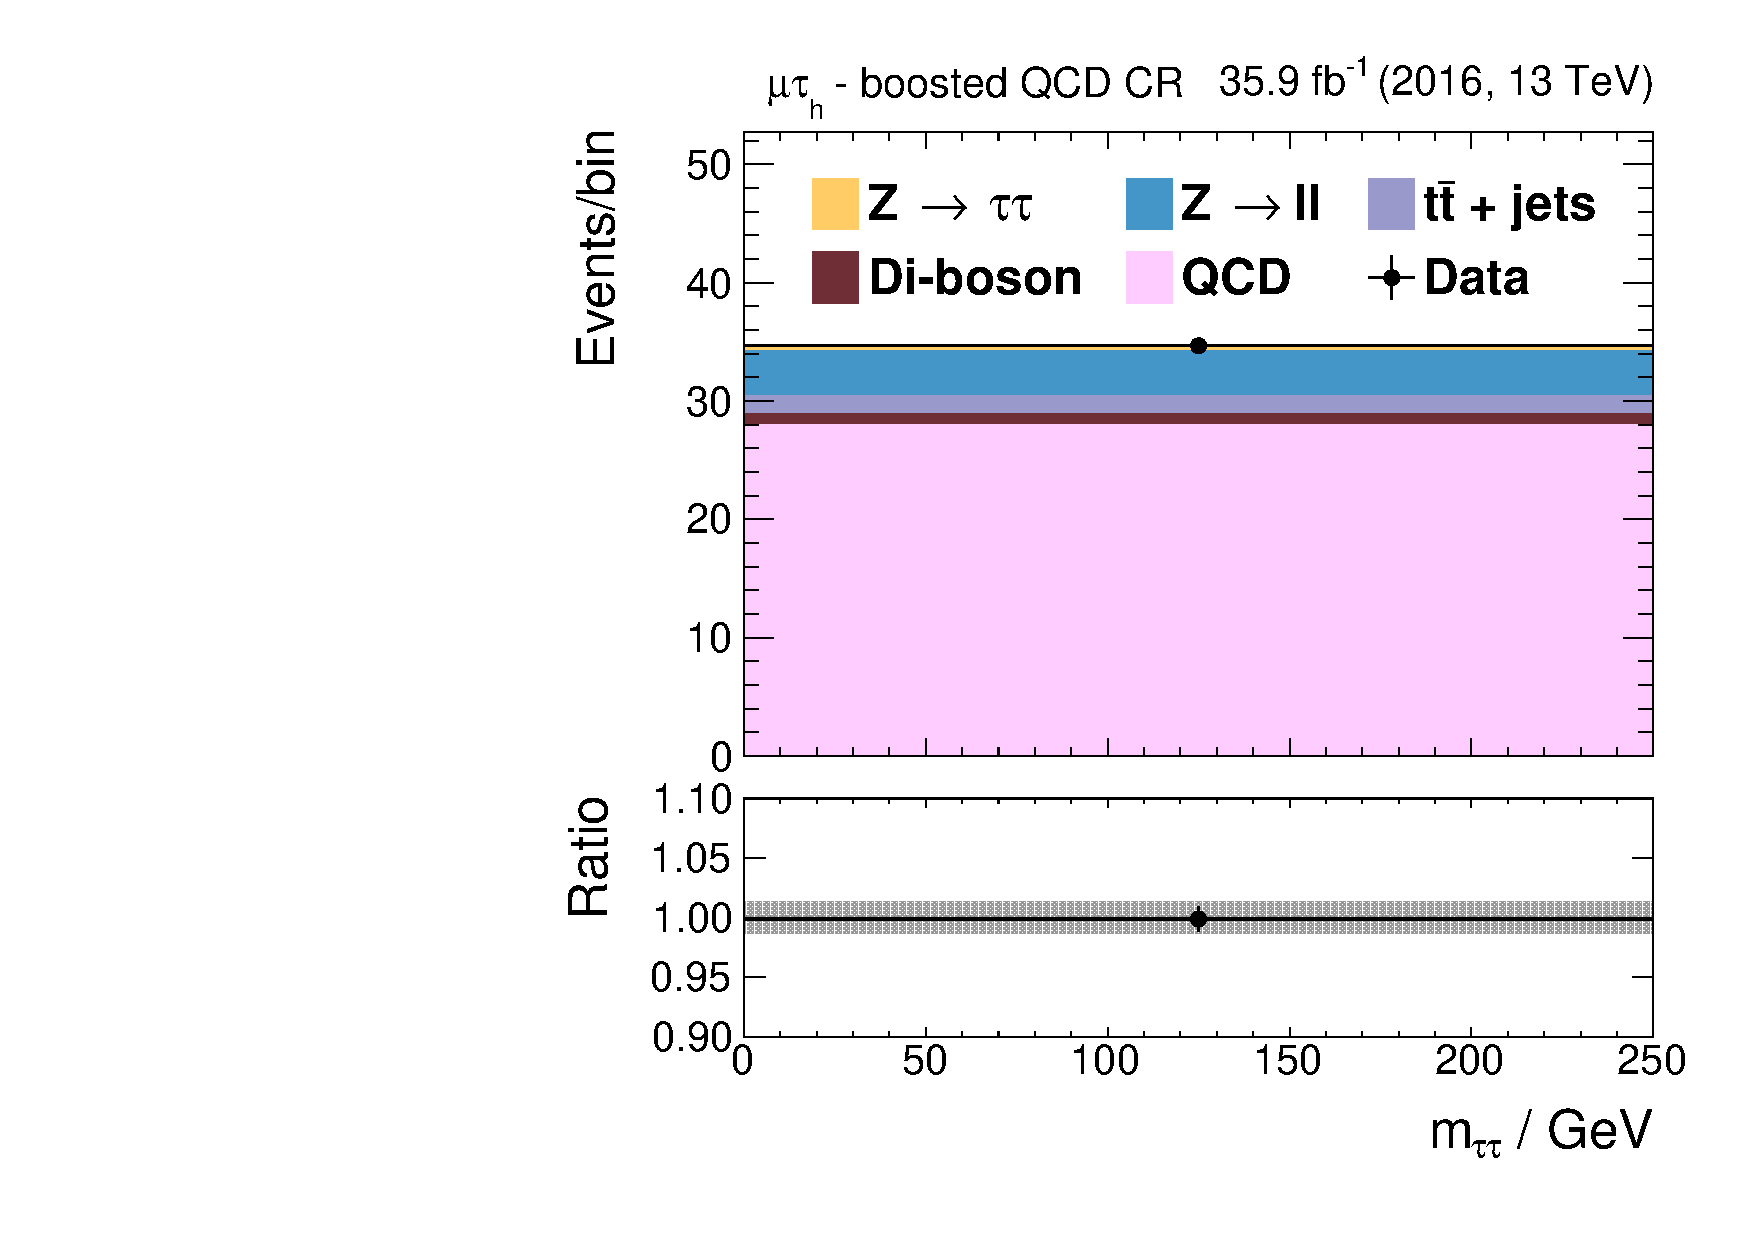
\includegraphics[width=0.47\textwidth]{Figures/background_estimation/qcd_mt_control-regions/htt_inputmt14__htt_mt_14_13TeV.pdf} \\
     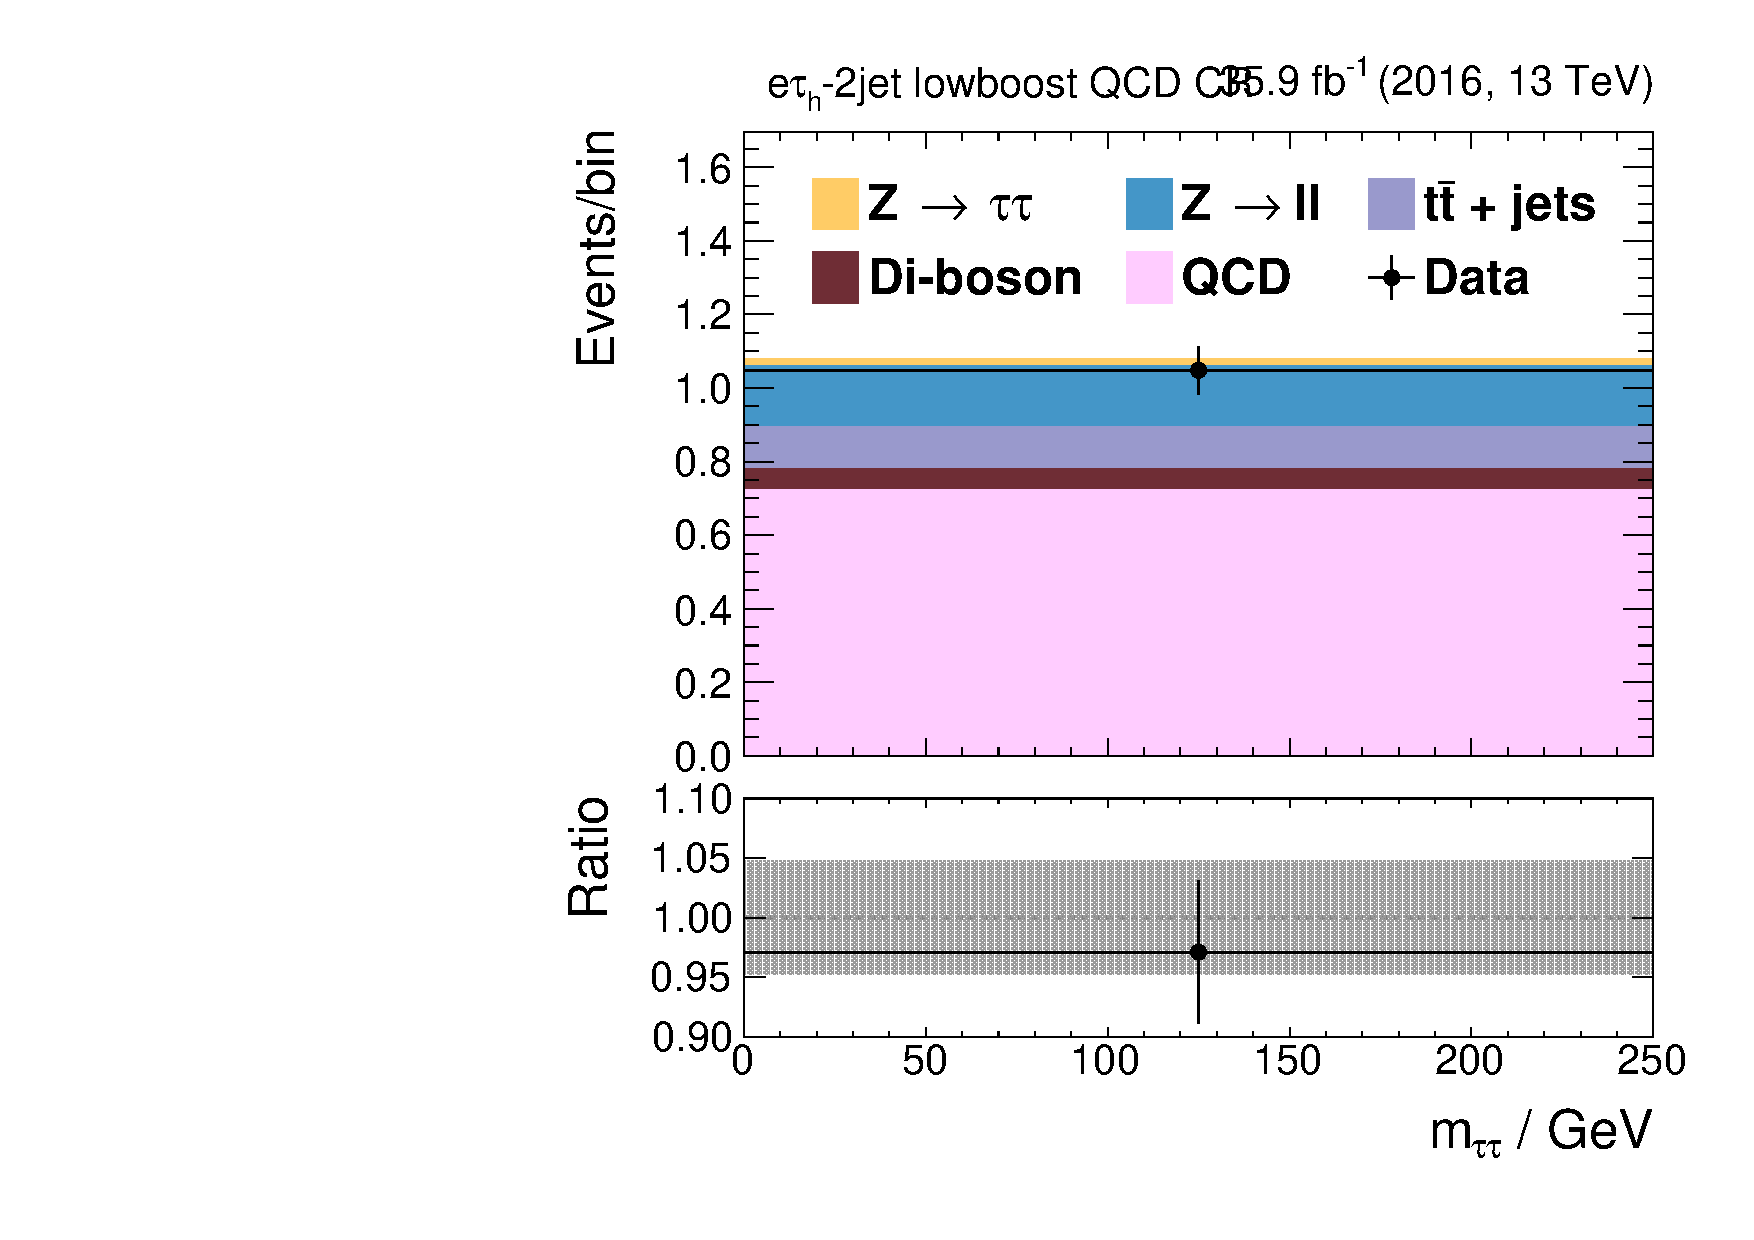
\includegraphics[width=0.47\textwidth]{Figures/background_estimation/qcd_et_control-regions/htt_inputet17__htt_et_17_13TeV.pdf}
     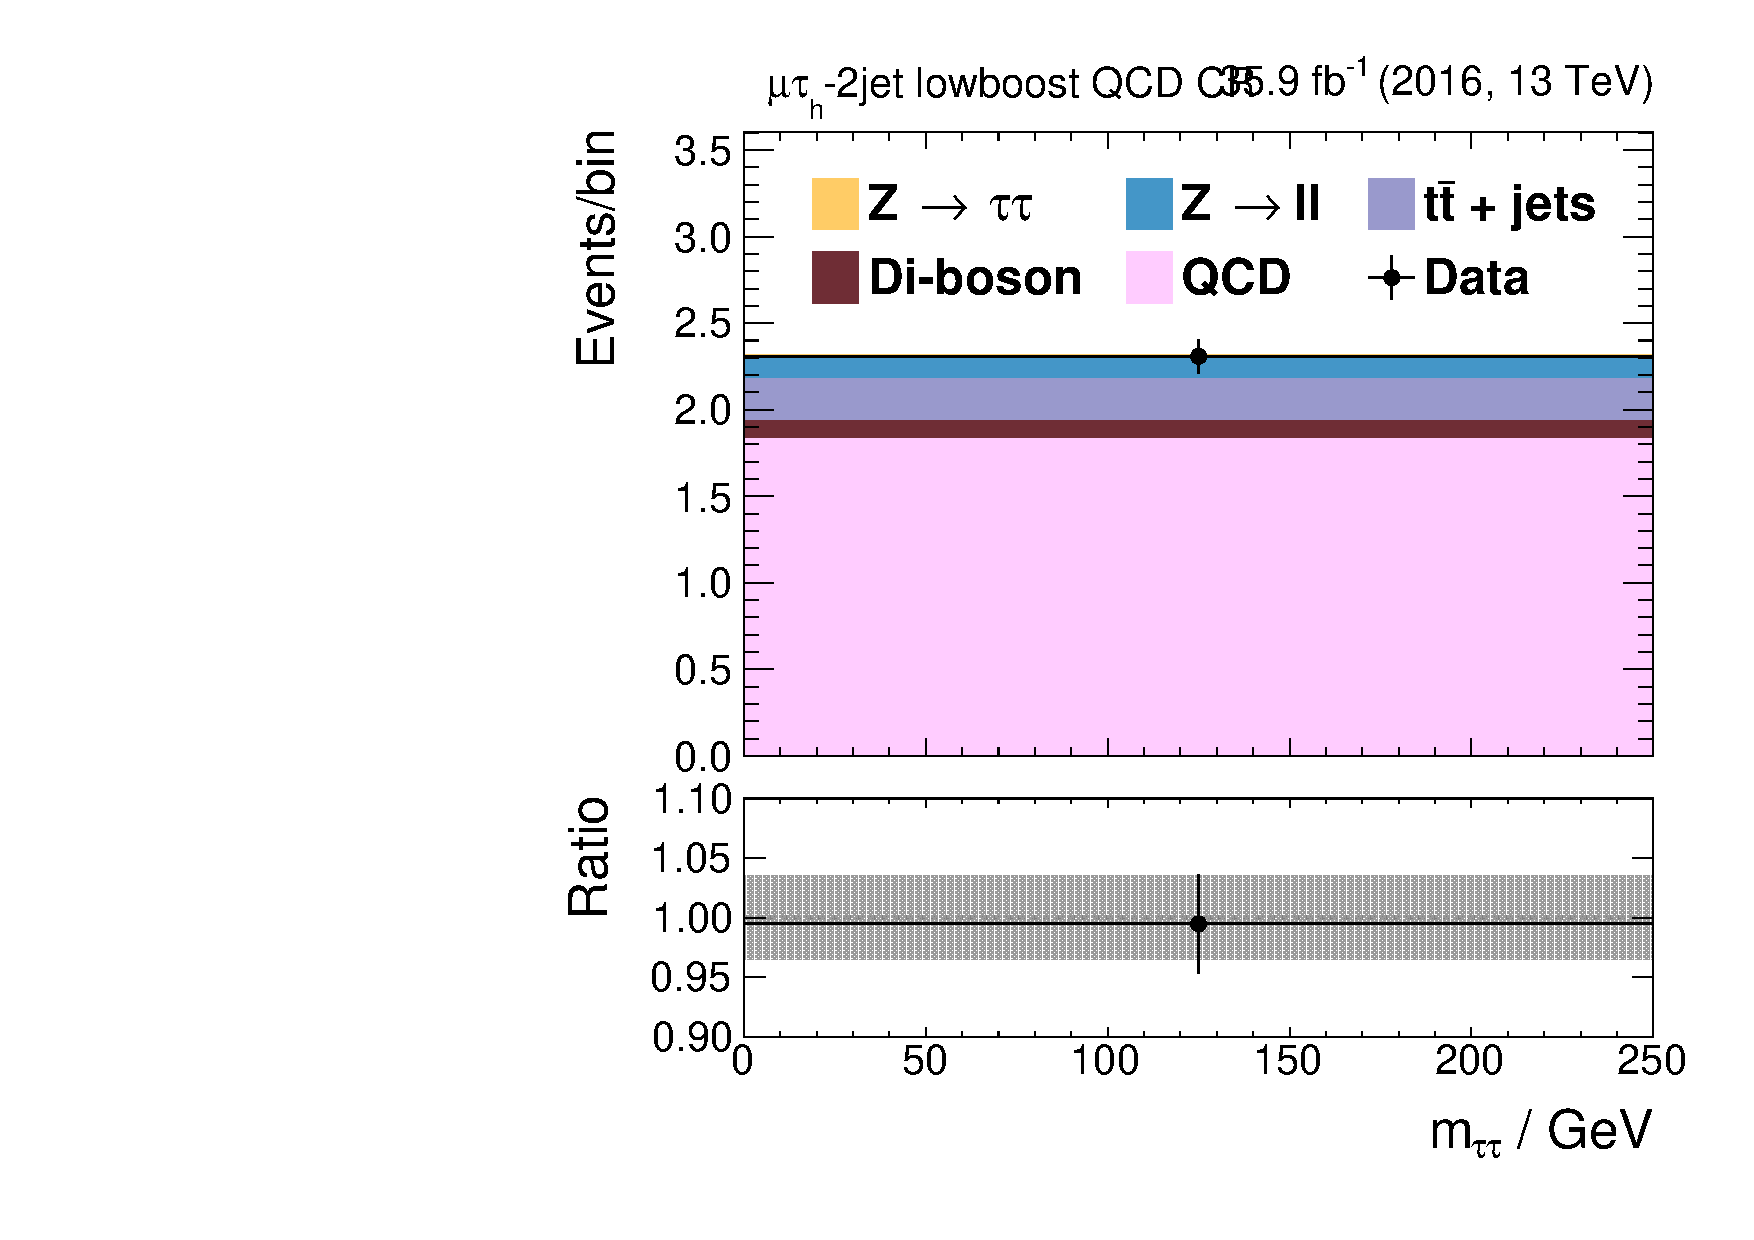
\includegraphics[width=0.47\textwidth]{Figures/background_estimation/qcd_mt_control-regions/htt_inputmt17__htt_mt_17_13TeV.pdf} 
  \caption[QCD control region in the \textit{boosted} and \textit{lowboosted} category.]{Background modeling and data in the QCD control region in the \textit{boosted} category (upper row) and the \textit{dijet lowboost} category (bottom row) for the $e\tau_\text{h}$ (left) and $\mu\tau_\text{h}$ (right) channel.}\label{supp_fig:etmtqcd:1jet_qcd_control}
 \end{figure}%

\clearpage
